\subsection{Anfälligkeit bei Adversarial Training}
Hier wird die Anfälligkeit der Modelle gegenüber \acrshort{uap}s während und nach dem Robustifizierungsprozess analysiert. 

\subsubsection{MRI Datensatz}
Die Generation von \acrshort{uap}s konnte auf vier der sechs Modelle, welche auf den MRI Datensatz trainiert wurden, erfolgreich erschwert werden. Bei diesen Modellen ist zu erkennen, dass die Generierungszeit eines \acrshort{uap}s über den Robustifizierungsdurchlauf zugenommen hat, bis es schlussendlich das erwünschte Abbruchkriterium, das Erreichen der gewünschten Mindesttäuschungsrate $r$, des \acrshort{uap}-Algorithmus nicht erreichen konnte. Hier sollte jedoch beachtet werden, dass der gewählte Regularisierungsparameter dieser Modelle, wie in Tabelle \ref{tab:Regularisierungsparameter}
ersichtlich, sehr hoch gewählt wurde. 

\begin{figure}[H]
    \centering
    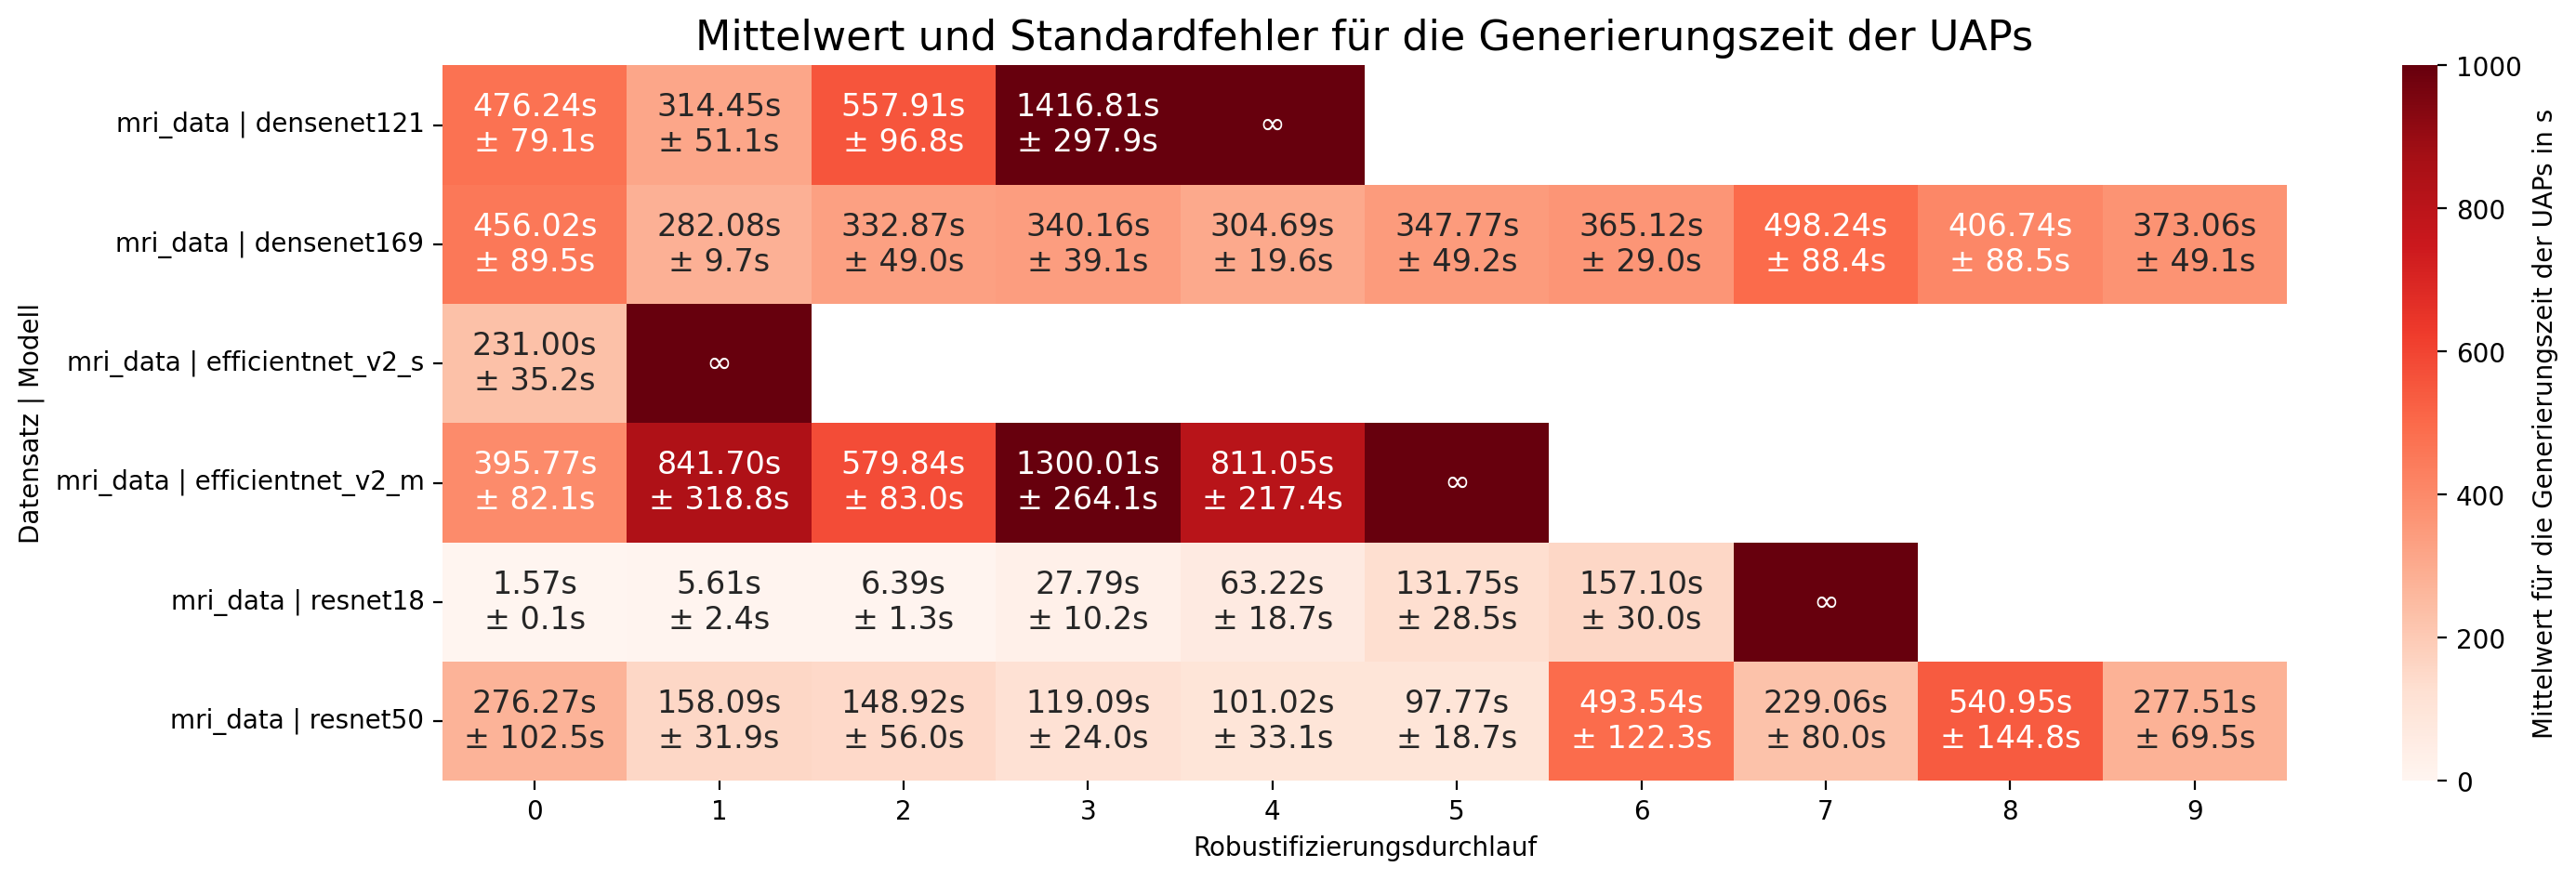
\includegraphics[width=\linewidth]{01-images/05-resultate/Generieungszeit MRI.png}
    \caption{Mittelwert und Standardfehler für die Generierungszeit der \acrshort{uap}s beim MRI Datensatz in Sekunden}
    \label{fig:GenerierungszeitUAPsMRI}
\end{figure}

%%%%%%
\paragraph{DenseNet}
In diesem Abschnitt werden die \acrlong{uap}s (\acrshort{uap}) über verschiedene Stufen der \Gls{robustifizierung} visualisiert. Die Analyse konzentriert sich auf die Modelle DenseNet121 und DenseNet169, die auf einem Hirntumor Datensatz trainiert wurden. In beiden Modellen konnte der Robustifizierungsprozess nur bis zur vierten Stufe durchgeführt werden. Aus diesem Grund existieren auch nur vier \acrshort{uap}s für jede Modellarchitektur.

% DenseNet121
\begin{figure}[H]
    \centering
    \foreach \y in {4} {%
        \text{Entwicklung der UAP (Index \y) durch Adversarial Attack und Adversarial Training}\\
        \foreach \x in {0,...,3} {%
            \ifnum\x>0 \hfill \fi 
            \begin{subfigure}{0.095\linewidth}
                \centering
                \includegraphics[height=\linewidth]{01-images/05-resultate/uap_densenet121/uap\y-densenet121-mri_data-n200-robustificationslevel\x.png}
            \end{subfigure}%
        }
    }
    \caption{UAPs der mit DenseNet121 trainierten Hirntumor Datensatz nach jedem Robustifikationslevel durch Adversarial Training von links nach rechts}
    \label{fig:uap-densenet121-hirntumor}
\end{figure}

In Abbildung \ref{fig:uap-densenet121-hirntumor} sind im zentralen Bereich negative Pixelwerte zu sehen, die durch eine blaue Färbung dargestellt werden. Diese negativen Werte verstärken sich mit zunehmendem Grad der \Gls{robustifizierung}. Besonders in der letzten Stufe der \Gls{robustifizierung} ist eine deutliche Konzentration negativer Perturbationen im Zentrum sichtbar. Links und rechts vom Zentrum zeigt sich ein abwechselndes Muster von hellen und dunklen Perturbationswerten, das über alle Robustifizierungsstufen hinweg konsistent bleibt. In der letzten Stufe der \Gls{robustifizierung} ist zudem eine erhöhte Intensität der Perturbationen im unteren Bereich der \acrshort{uap} zu erkennen, was zu einem auffälligen roten Fleck führt. Diese Beobachtungen deuten darauf hin, dass Angriffe zunächst im zentralen Bereich der Bilder besonders effektiv sind und sich mit zunehmender \Gls{robustifizierung} allmählich in Richtung der Bildränder ausbreiten.

% DenseNet169
\begin{figure}[H]
    \centering
    \foreach \y in {0} {%
        \text{Entwicklung der UAP (Index \y) durch Adversarial Attack und Adversarial Training}\\
        \foreach \x in {0,...,3} {%
            \ifnum\x>0 \hfill \fi 
            \begin{subfigure}{0.095\linewidth}
                \centering
                \includegraphics[height=1\linewidth]{01-images/05-resultate/uap_densenet169/uap\y-densenet169-mri_data-n200-robustificationslevel\x.png}
            \end{subfigure}%
        }
    }
    \caption{UAPs der mit DenseNet169 trainierten Hirntumor Datensatz nach jedem Robustifikationslevel durch Adversarial Training von links nach rechts}
    \label{fig:uap-densenet169-hirntumor}
\end{figure}

In Abbildung \ref{fig:uap-densenet169-hirntumor} zeigen die universellen Adversarial Perturbationen (\acrshort{uap}) über alle Robustifikationsstufen hinweg eine auffallende Ähnlichkeit. Wie beim kleineren Modell DenseNet121 konzentrieren sich die negativen Perturbationswerte deutlich im zentralen Bereich, während die positiven Perturbationswerte hauptsächlich in den Randbereichen auftreten. Auffällig ist auch, dass bei der letzten \acrshort{uap} eine horizontale, wechselnde Struktur der Perturbationen ausserhalb des Zentrumsbereichs erkennbar ist, die ebenfalls im kleineren Modell beobachtet werden kann.

\paragraph{EfficientNet}
In diesem Abschnitt betrachten wir die \acrshort{uap}, die aus den mit EfficientNet trainierten Modellen auf Hirntumordaten generiert wurden.

% EfficientNet-V2-S
\begin{figure}[H]
    \centering
    \foreach \y in {2} {%
        \text{Entwicklung der UAP (Index \y) durch Adversarial Attack und Adversarial Training}\\
        \foreach \x in {0,...,0} {%
            \ifnum\x>0 \hfill \fi 
            \begin{subfigure}{0.095\linewidth}
                \centering
                \includegraphics[height=1\linewidth]{01-images/05-resultate/uap_efficientnet_s/uap\y-efficientnet_v2_s-mri_data-n200-robustificationslevel\x.png}
            \end{subfigure}%
        }
    }
    \caption{UAPs der mit EfficientNetV2-S trainierten Hirntumor Datensatz nach jedem Robustifikationslevel durch Adversarial Training von links nach rechts}
    \label{fig:uap-efficientnetv2s-hirntumor}
\end{figure}

Beim Modell EfficientNetV2-S konnten nach der initialen \Gls{robustifizierung} keine weiteren universellen adversarialen Perturbationen (\acrshort{uap}) erzeugt werden. Diese spezifische \acrshort{uap} zeigt eine hohe Effektivität im adversarialen Training. Bei der Analyse der \acrshort{uap} ist kein eindeutiges Perturbationsmuster zu erkennen. Die Perturbationswerte sind am oberen sowie am linken und rechten Rand der \acrshort{uap} überwiegend positiv, während der untere Rand keine auffälligen Perturbationswerte aufweist. Das Zentrum des Bildes weist eine Mischung aus positiven und negativen Perturbationen auf. Am oberen Rand der \acrshort{uap} ist eine negative, blaue Perturbationslinie zu beobachten. Insgesamt ist das Muster der Perturbationen schwer zu beschreiben, da sie über die gesamte Heatmap verstreut sind und kein spezifisches Muster, wie beim DenseNet Modell, aufweisen.

% EfficientNet-V2-M
\begin{figure}[H]
    \centering
    \foreach \y in {1} {%
        \text{Entwicklung der UAP (Index \y) durch Adversarial Attack und Adversarial Training}\\
        \foreach \x in {0,...,4} {%
            \ifnum\x>0 \hfill \fi 
            \begin{subfigure}{0.095\linewidth}
                \centering
                \includegraphics[height=1\linewidth]{01-images/05-resultate/uap_efficientnet_m/uap\y-efficientnet_v2_m-mri_data-n200-robustificationslevel\x.png}
            \end{subfigure}%
        }
    }
    \caption{UAPs der mit EfficientNetV2-M trainierten Hirntumor Datensatz nach jedem Robustifikationslevel durch Adversarial Training von links nach rechts}
    \label{fig:uap-efficientnetv2m-hirntumor}
\end{figure}

Die universellen adversarialen Perturbationen (\acrshort{uap}) des Modells EfficientNetV2-M, das auf dem Hirntumor-Datensatz trainiert wurde, weisen über fünf Robustifikationslevel hinweg einheitliche vertikale Muster auf der rechten Seite der \acrshort{uap} auf. Diese vertikalen Muster sind durch hohe positive Perturbationswerte im gesamten \acrshort{uap} gekennzeichnet. Negative Perturbationswerte treten tendenziell in der oberen Hälfte der \acrshort{uap} auf. Der untere Teil der \acrshort{uap} wird erst durch zunehmende Robustifikation betroffen. Mit steigenden Robustifikationsleveln scheint sich das vertikale Perturbationsmuster zu verlängern.

\paragraph{ResNet}
Hier in diesem Abschnitt visualisieren wir die \acrshort{uap}, die aus dem ResNet trainierten Hirntumor Daten generiert und robustifiziert wurden. 

\begin{figure}[H]
    \centering
    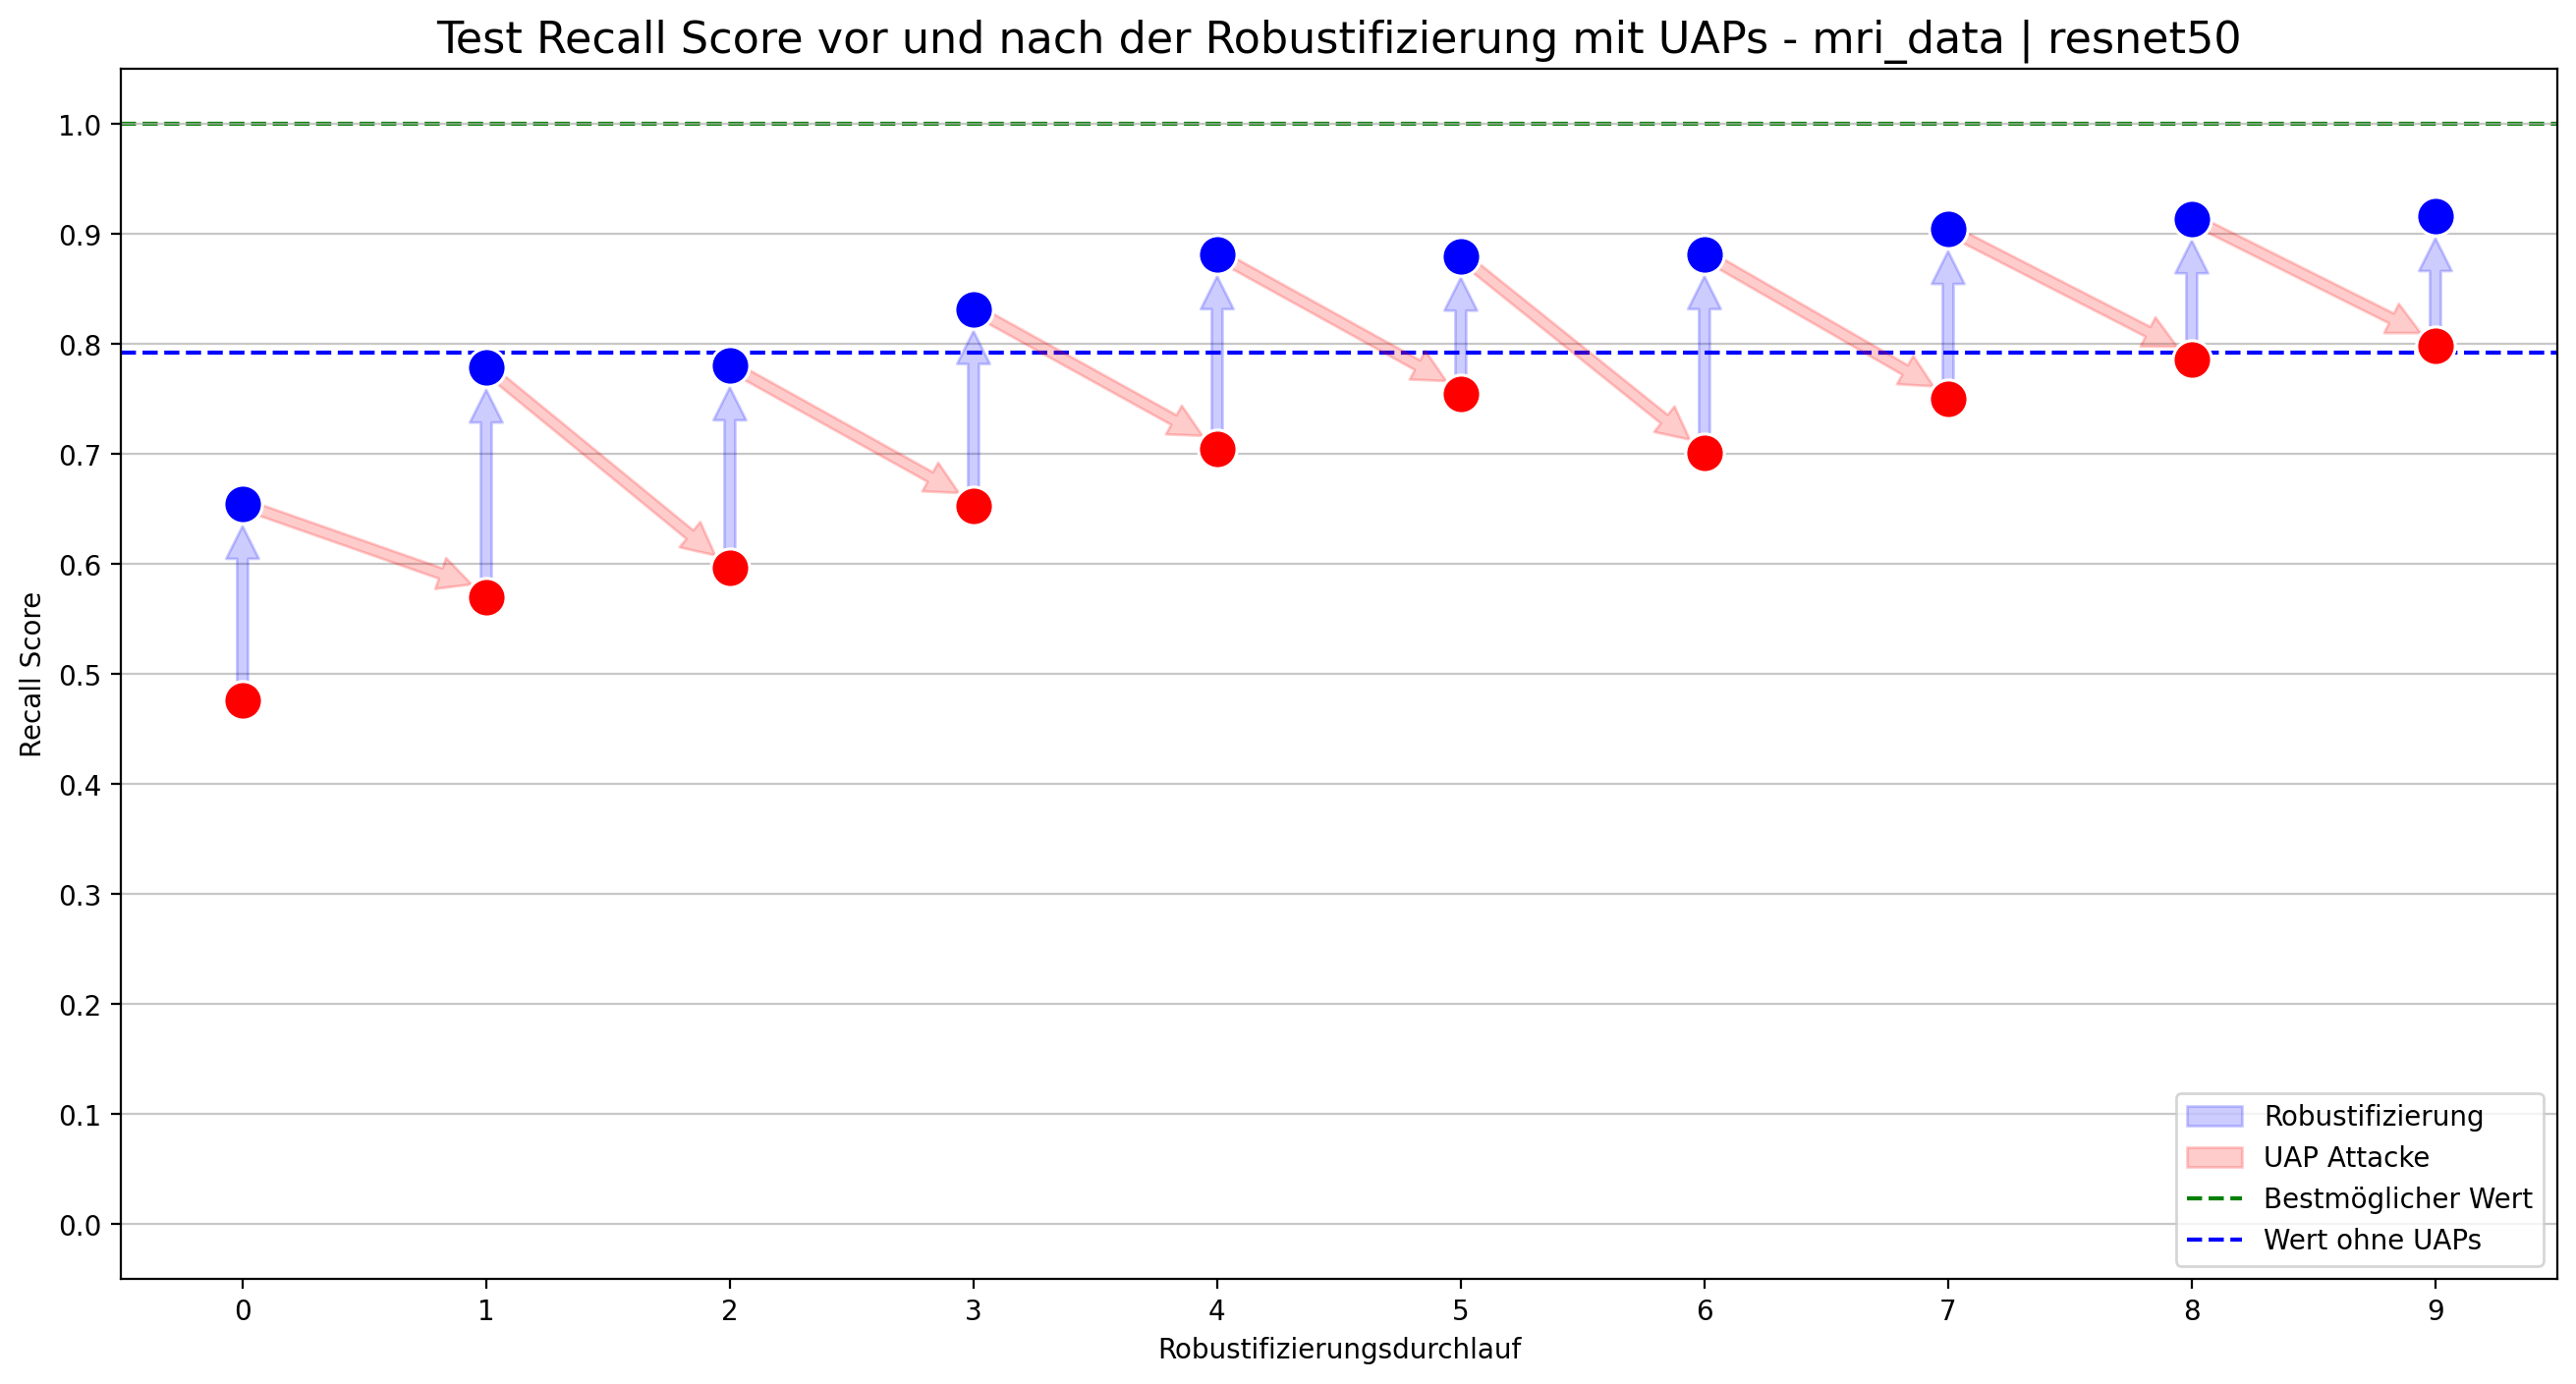
\includegraphics[width=\linewidth]{01-images/05-resultate/RecallRobustification_MRI_ResNet50.png}
    \caption{Verlauf der Recall Metrik pro Robustifikationsschritt für das Modell ResNet50}
    \label{fig:RecallRobustification MRI ResNet50}
\end{figure}

Die Visualisierung des Verlaufs der Recall-Metrik während des Robustifizierungsprozesses des ResNet50-Modells zeigt einen Anstieg des Recall-Wertes mit \acrshort{uap}s nach jedem Robustifizierungsdurchlauf. Allerdings bleibt das Modell bei der Generierung neuer \acrshort{uap}s weiterhin vulnerabel, was zu einem erneuten Absinken der Recall-Metrik führt. Über die Robustifizierungsdurchläufe hinweg ist jedoch ein tendenzieller Anstieg des Recalls zu beobachten, was auf eine erfolgreiche Reduzierung von False-Negatives nach mehreren Robustifizierungsdurchläufen hindeutet.

\begin{figure}[H]
    \centering
    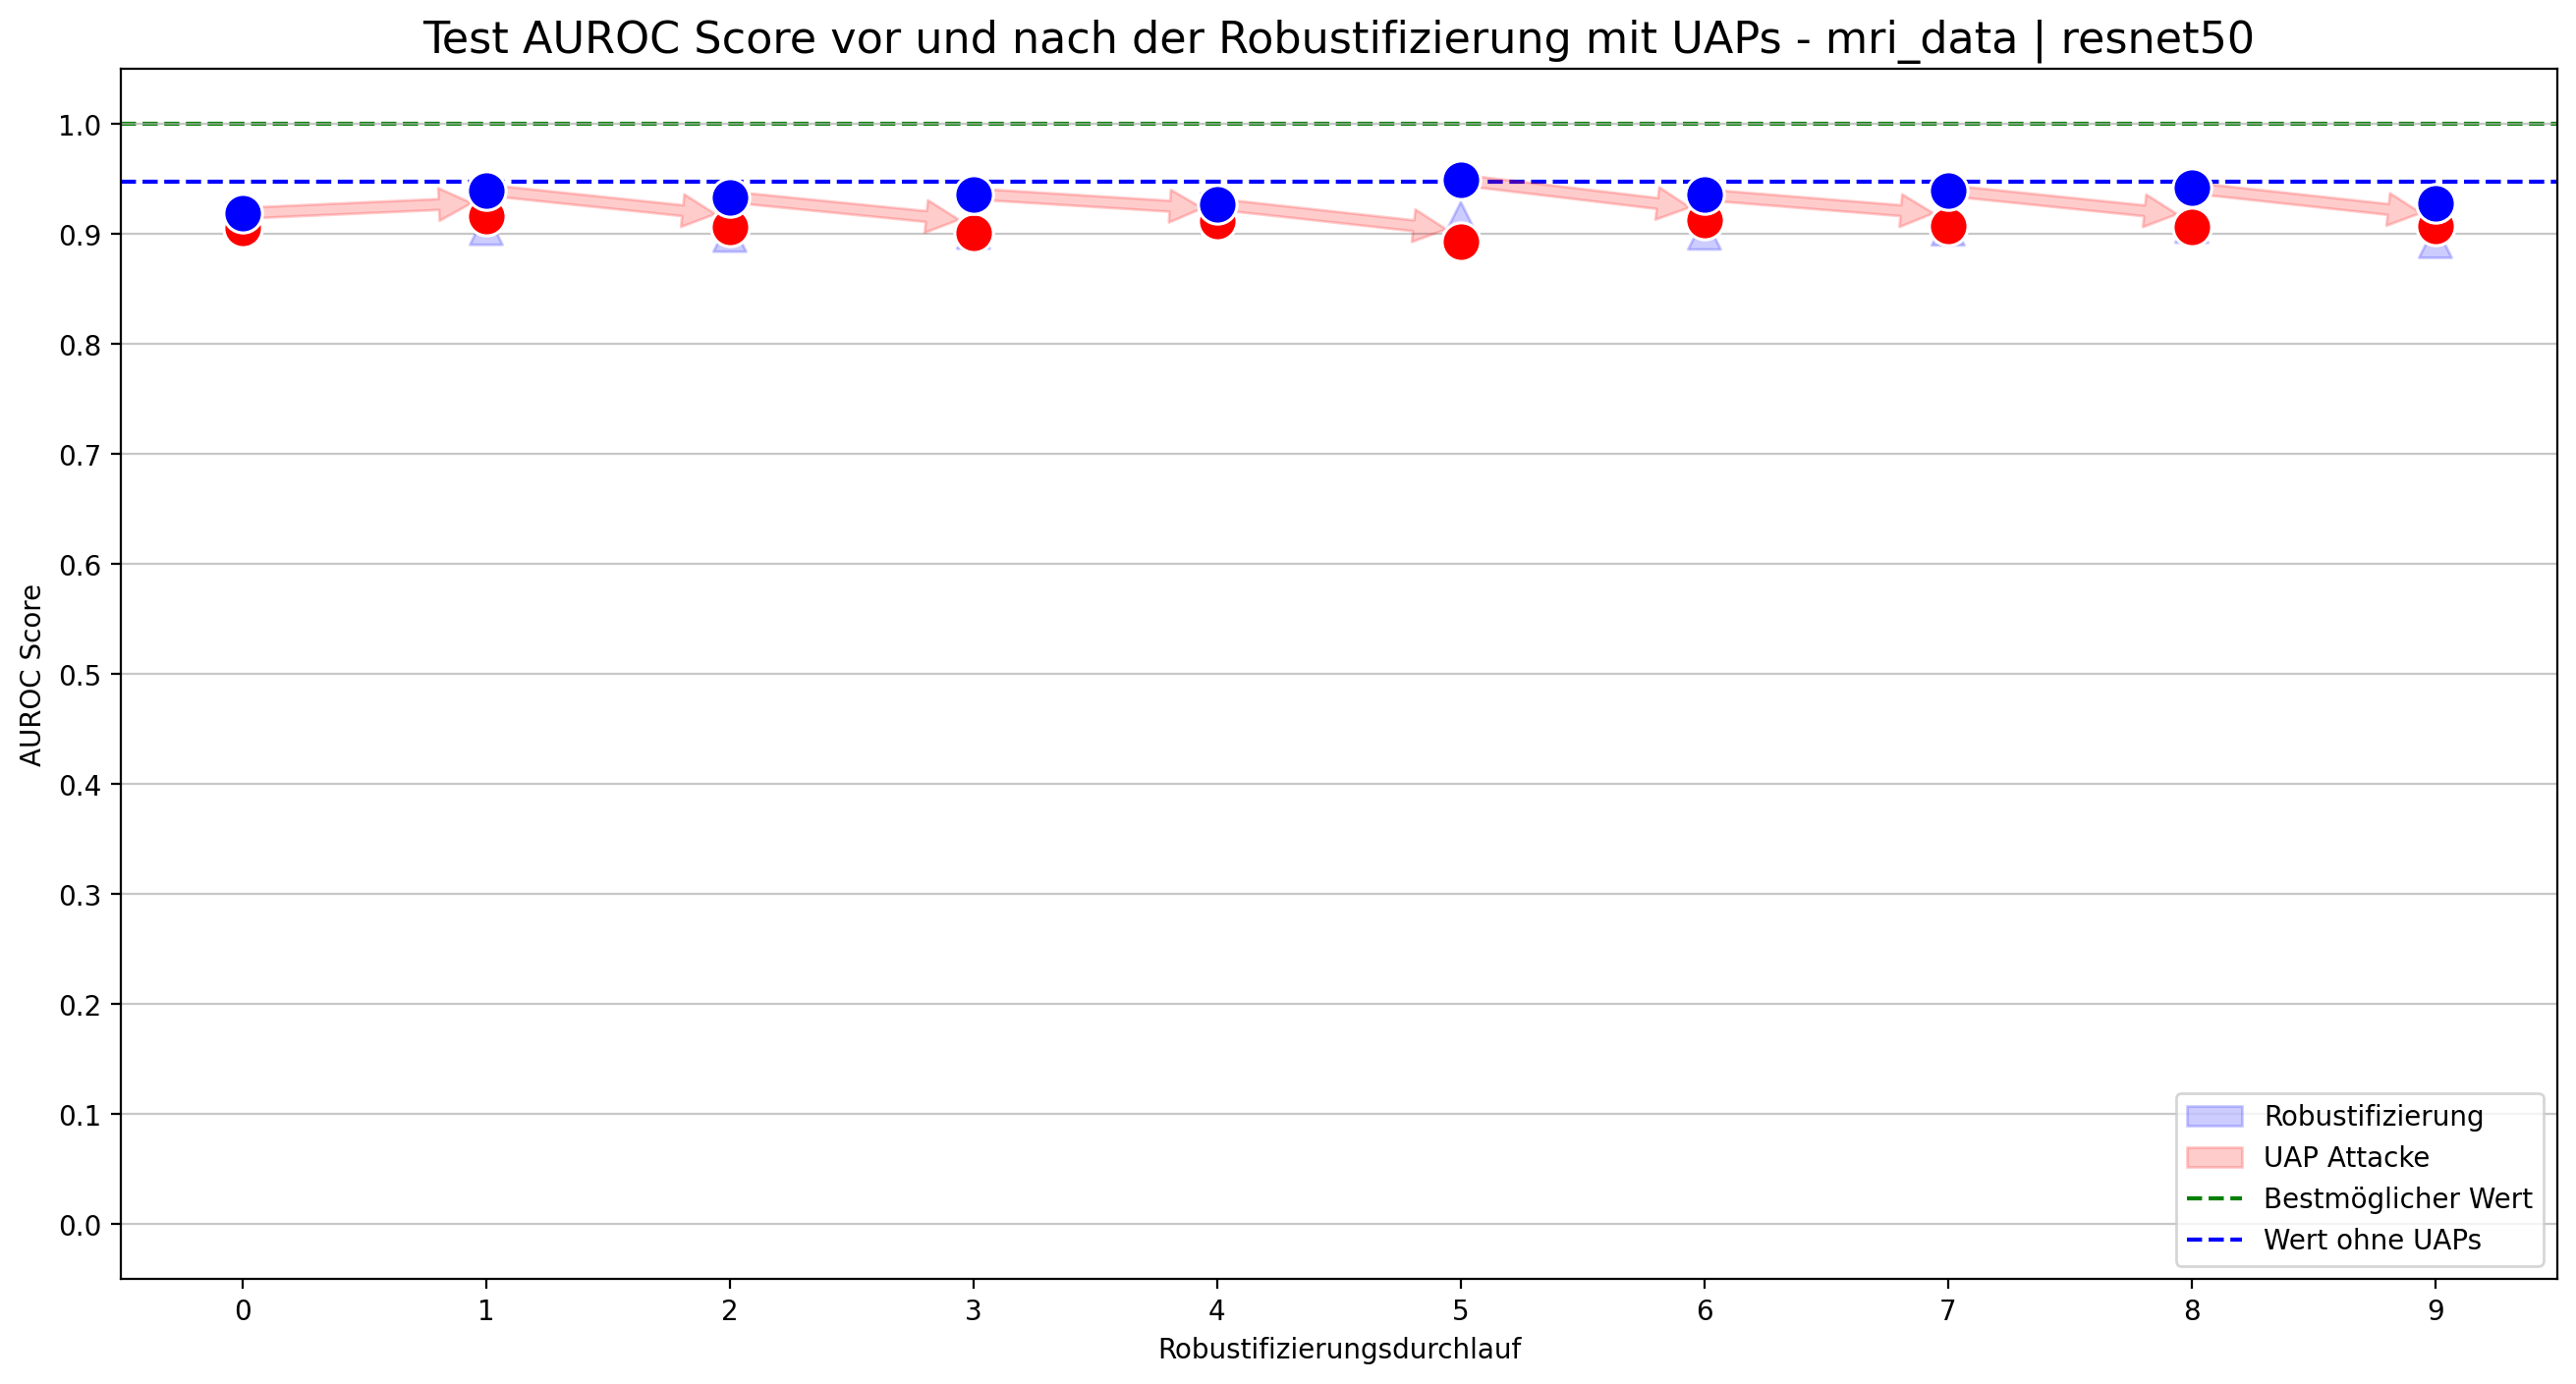
\includegraphics[width=\linewidth]{01-images/05-resultate/AUROCRobustification_MRI_ResNet50.png}
    \caption{Verlauf der AUROC Metrik pro Robustifikationsschritt für das Modell ResNet50}
    \label{fig:AUROCRobustification MRI ResNet50}
\end{figure}

Im Vergleich dazu zeigt die AUROC-Metrik keine signifikante Verschlechterung trotz des Anstiegs der Recall-Metrik. Dies deutet auf eine ausgewogene Verbesserung der Modellleistung hin.

\begin{figure}[H]
    \centering
    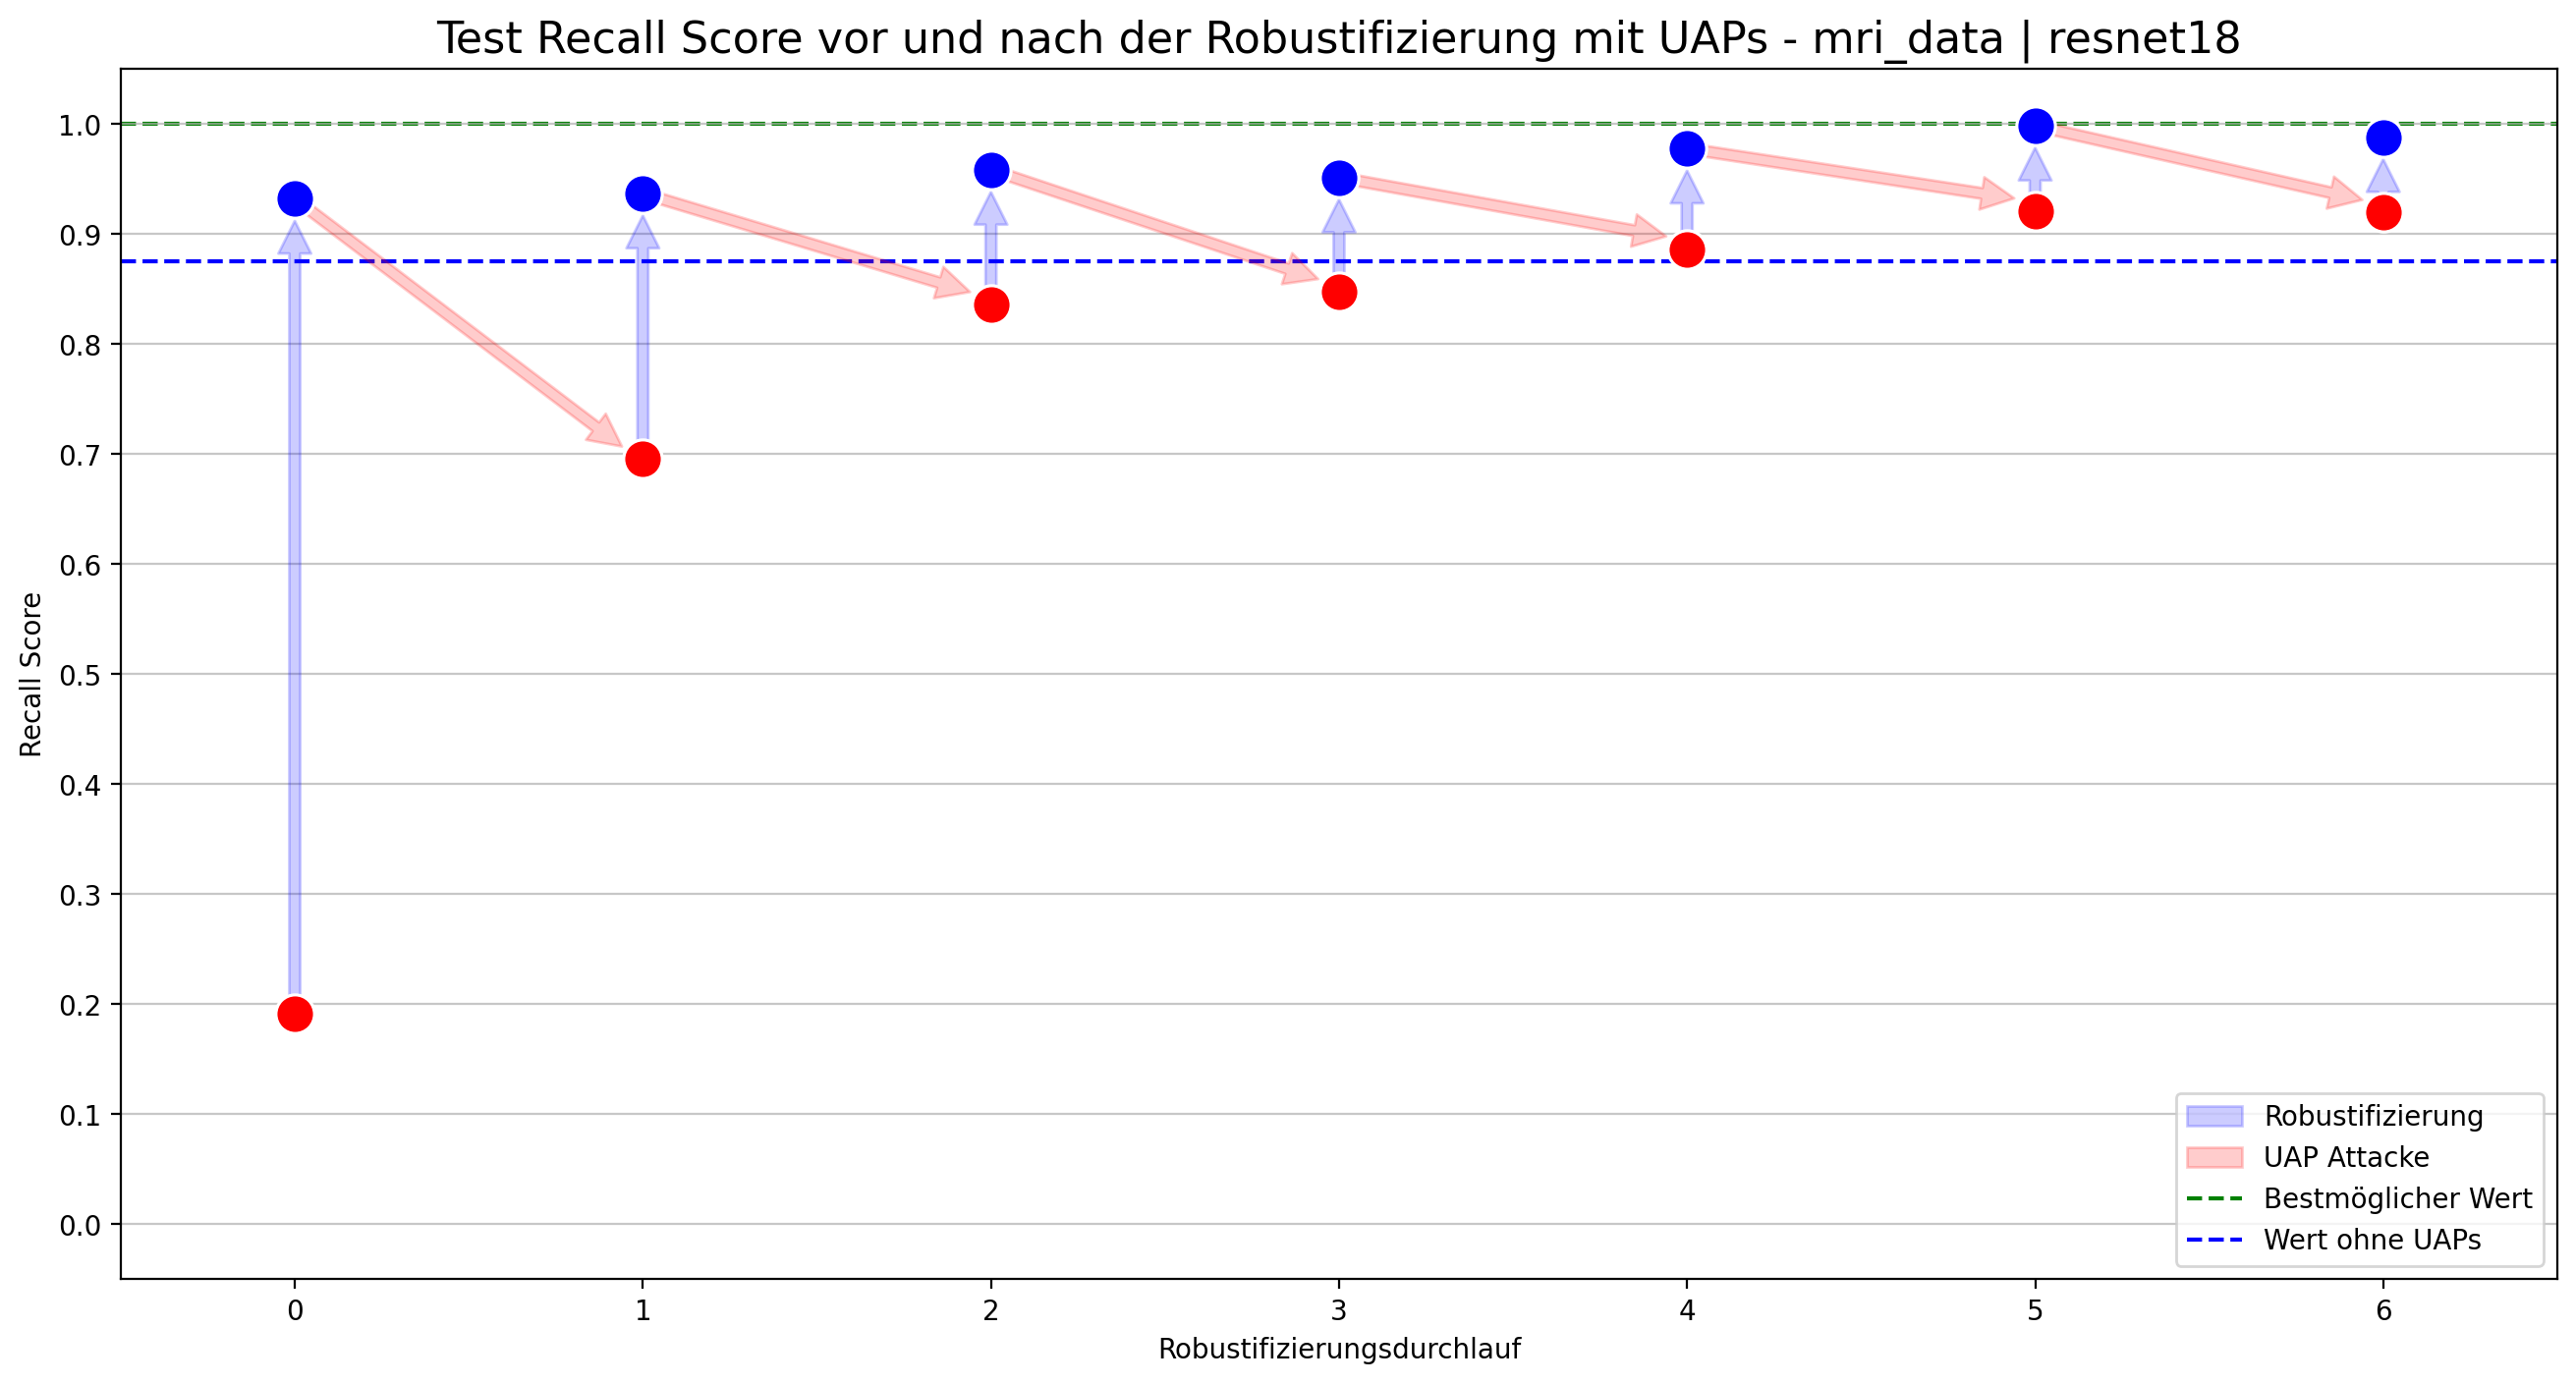
\includegraphics[width=\linewidth]{01-images/05-resultate/RecallRobustification_MRI_ResNet18.png}
    \caption{Verlauf der Recall Metrik pro Robustifikationsschritt für das Modell ResNet18}
    \label{fig:RecallRobustification MRI ResNet18}
\end{figure}

Im Vergleich zum ResNet50-Modell zeigt der Robustifizierungsverlauf des ResNet18-Modells ein ähnliches, jedoch ausgeprägteres Muster. Die \Gls{robustifizierung} scheint hier besonders effektiv in der Reduzierung von False-Negatives zu sein.

\begin{figure}[H]
    \centering
    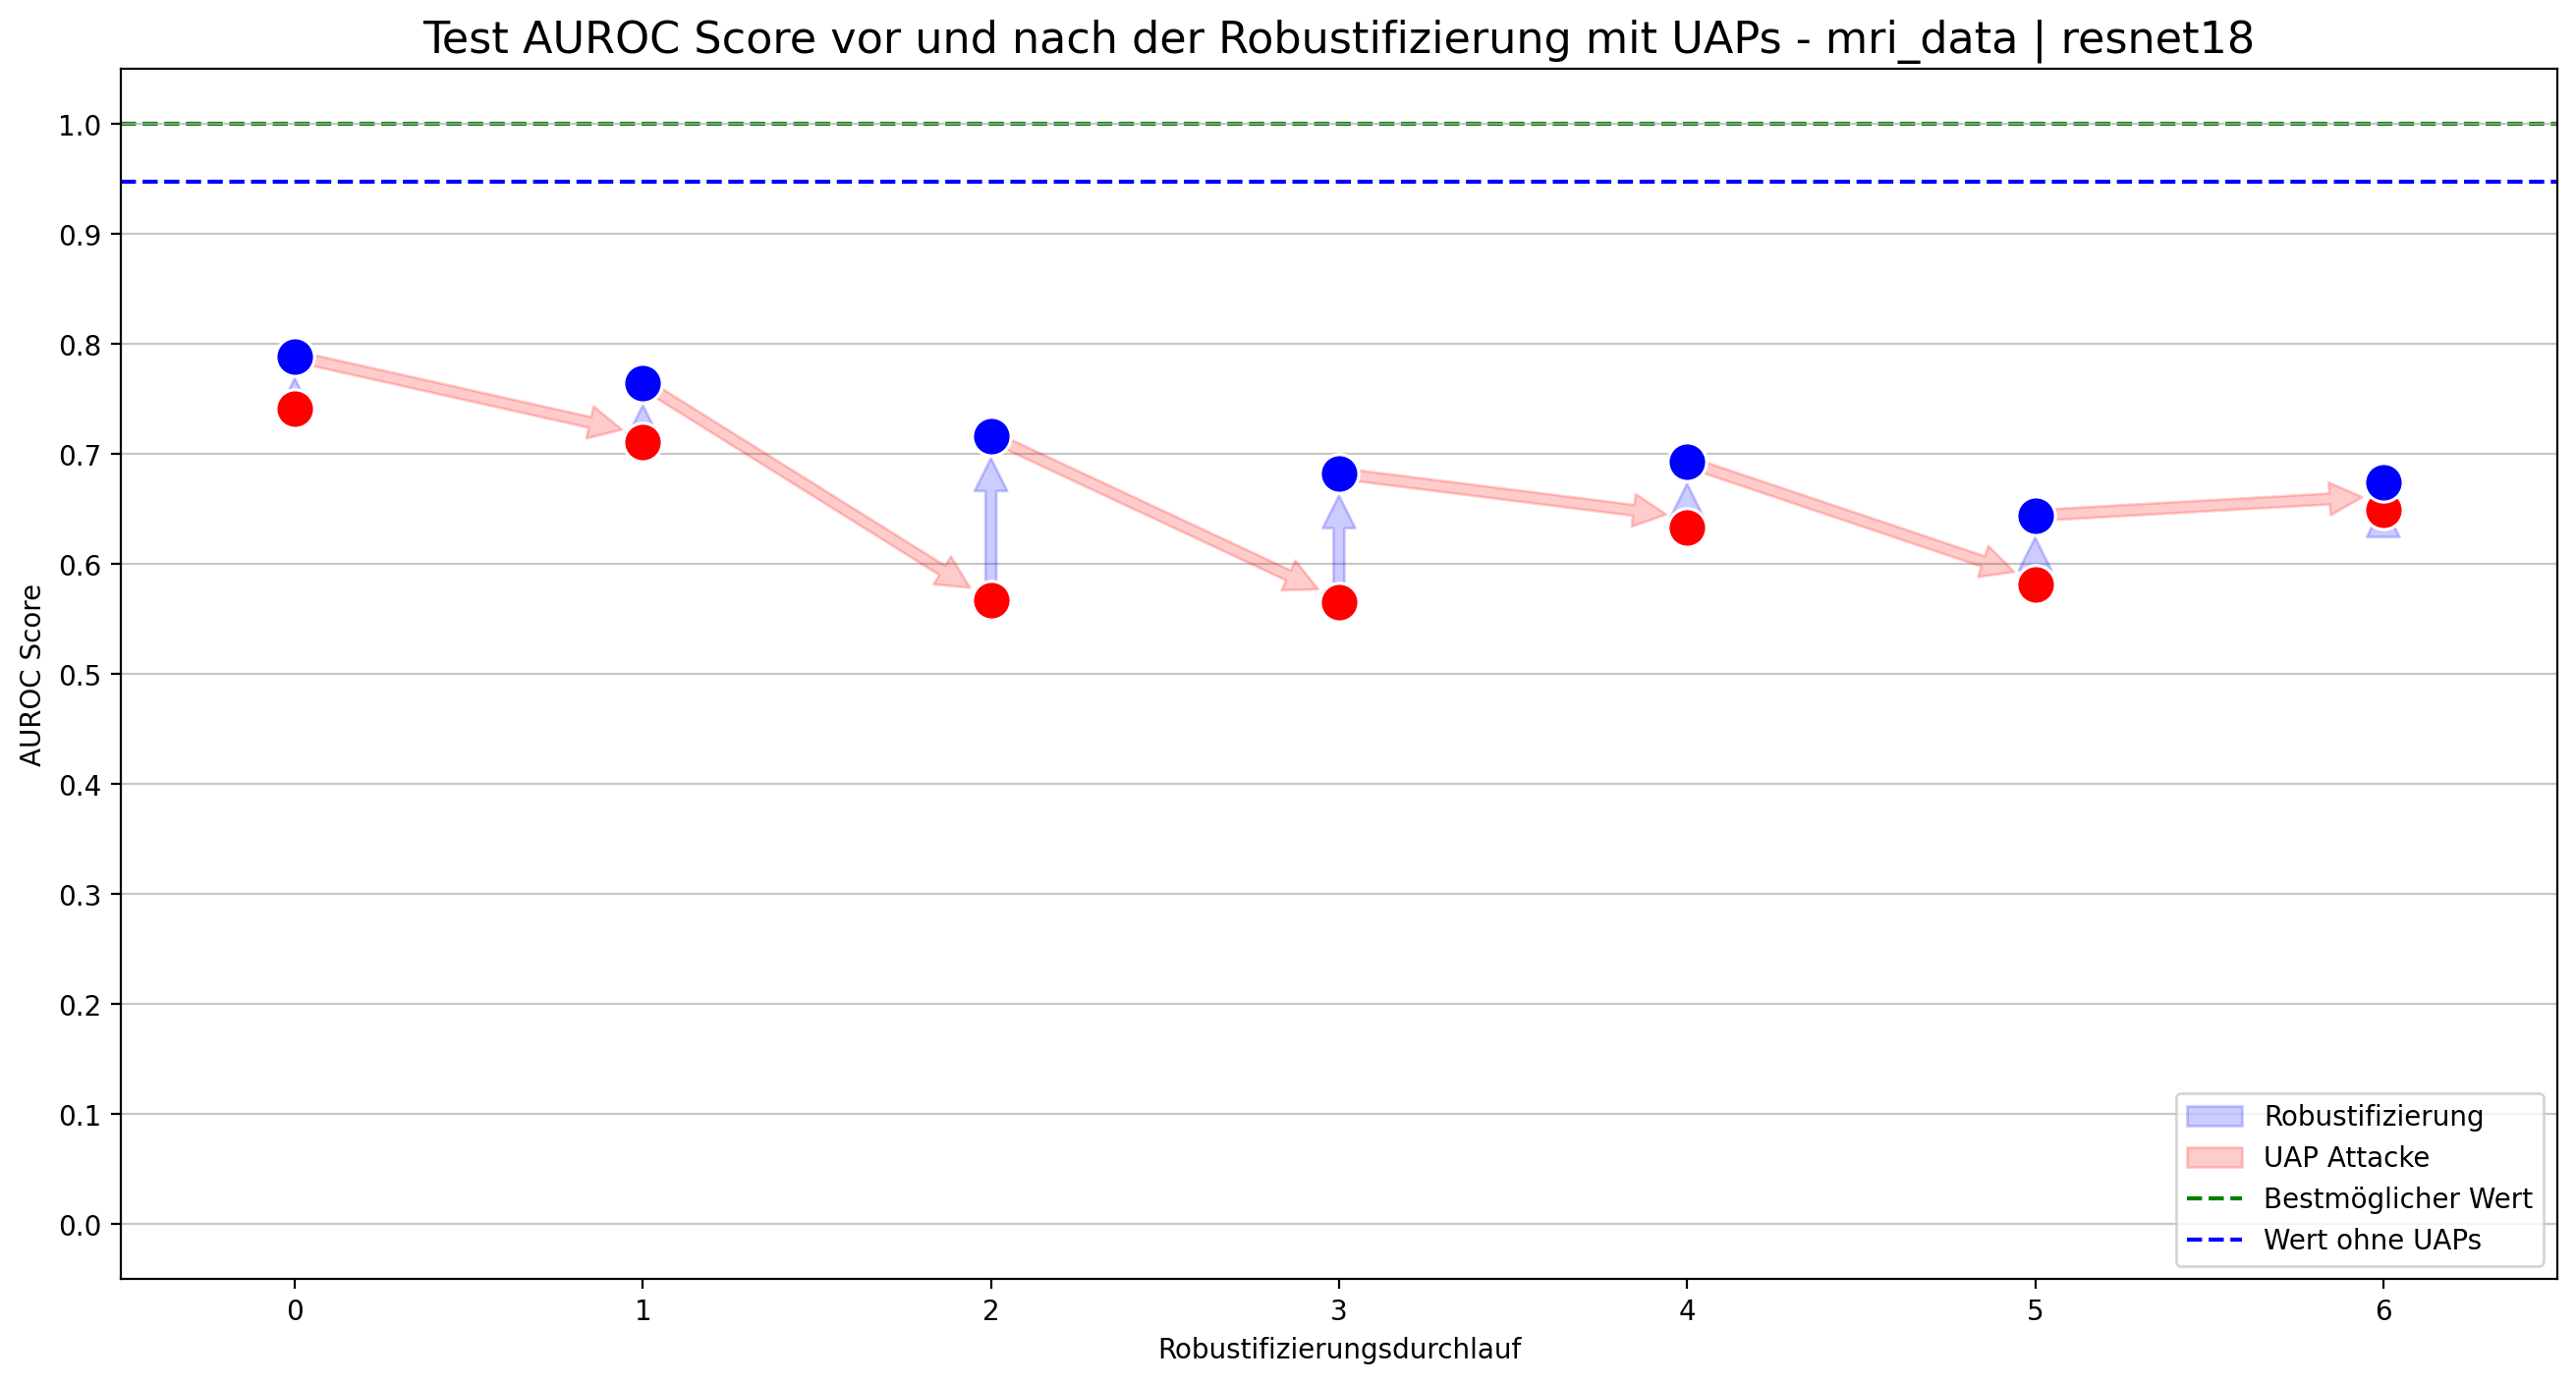
\includegraphics[width=\linewidth]{01-images/05-resultate/AUROCRobustification_MRI_ResNet18.png}
    \caption{Verlauf der AUROC Metrik pro Robustifikationsschritt für das Modell ResNet18}
    \label{fig:AUROCRobustification MRI ResNet18}
\end{figure}

Eine genauere Betrachtung der AUROC-Metrik offenbart jedoch, dass diese während des Robustifizierungsverlauf sinkt. Dies legt nahe, dass das ResNet18-Modell möglicherweise eine Tendenz entwickelt, generell weniger negative Vorhersagen zu treffen, anstatt tatsächlich zu lernen, mit den Perturbationen umzugehen.

% ResNet18
\begin{figure}[H]
    \centering
    \foreach \y in {1} {%
        \text{Entwicklung der UAP (Index \y) durch Adversarial Attack und Adversarial Training}\\
        \foreach \x in {0,...,6} {%
            \ifnum\x>0 \hfill \fi 
            \begin{subfigure}{0.095\linewidth}
                \centering
                \includegraphics[height=1\linewidth]{01-images/05-resultate/uap_resnet18/uap\y-resnet18-mri_data-n200-robustificationslevel\x.png}
            \end{subfigure}%
        }
    }
    \caption{UAPs der mit ResNet18 trainierten Hirntumor Datensatz nach jedem Robustifikationslevel durch Adversarial Training von links nach rechts}
    \label{fig:uap-resnet18-hirntumor}
\end{figure}

Die Perturbationen im ResNet18-Modell unterscheiden sich deutlich von denen, die in den bisherigen Beobachtungen bei DenseNet- und EfficientNet-Modellen festgestellt wurden. Die Perturbationen, sowohl positive als auch negative, sind über die gesamte \acrshort{uap} punktuell verteilt. Es ist klar erkennbar, dass die Perturbationen an den Rändern der \acrshort{uap} überwiegend positiv sind. Diese Tendenz bleibt über verschiedene Robustifikationslevel hinweg bestehen, wenn auch in unterschiedlicher Intensität. Insgesamt zeigen die Perturbationen im ResNet18-Modell auf dem Hirntumor-Datensatz ein punktuelles Muster.

% ResNet50
\begin{figure}[H]
    \centering
    \foreach \y in {3} {%
        \text{Entwicklung der UAP (Index \y) durch Adversarial Attack und Adversarial Training}\\
        \foreach \x in {0,...,9} {%
            \ifnum\x>0 \hfill \fi 
            \begin{subfigure}{0.095\linewidth}
                \centering
                \includegraphics[height=1\linewidth]{01-images/05-resultate/uap_resnet50/uap\y-resnet50-mri_data-n200-robustificationslevel\x.png}
            \end{subfigure}%
        }
    }
    \caption{UAPs der mit ResNet50 trainierten Hirntumor Datensatz nach jedem Robustifikationslevel durch Adversarial Training von links nach rechts}
    \label{fig:uap-resnet50-hirntumor}
\end{figure}

Die universellen adversarialen Perturbationen (\acrshort{uap}) im ResNet50-Modell zeigen über alle Robustifikationslevel hinweg ein ähnliches Muster. Wie bereits beim ResNet18-Modell sind auch hier punktuelle Angriffe durch negative und positive Perturbationen zu beobachten. Allerdings erreichen die punktuell attackierten Perturbationen im ResNet50-Modell deutlich höhere Werte, was eine stärkere Beeinflussung des Eingabebildes zur Folge haben kann. Auffällig ist, dass im Zentrum des \acrshort{uap} sowohl negative als auch positive Perturbationen auftreten, während an den Rändern überwiegend positive Perturbationen zu finden sind.

\paragraph{Zusammenfassung}
In den Experimenten mit verschiedenen Klassifikationsmodellen wurden deutliche Unterschiede in den universellen adversarialen Perturbationen (\acrshort{uap}) beobachtet. Bei beiden DenseNet-Modellen, wurde festgestellt, dass das Zentrum der MRI-Bilder über alle Robustifikationslevel hinweg verstärkt durch negative Perturbationen attackiert wird. Diese zentrale negative Attacke wird von abwechselnden horizontalen Perturbationen umrahmt, die eine charakteristische Struktur im \acrshort{uap} bilden.

EfficientNet-Modelle zeigen hingegen ein konsistentes vertikales Muster in den Perturbationen. Diese vertikalen Linien durchziehen die \acrshort{uap}, unabhängig von der Grösse des Modells oder dem Robustifikationslevel. Die vertikalen Muster sind durch hohe positive Perturbationswerte gekennzeichnet, die sich über die rechte Seite des Bildes erstrecken.

Bei den ResNet-Modellen, insbesondere ResNet18 und ResNet50, treten punktuelle Perturbationen auf. Diese punktuellen Angriffe sind über das gesamte Bild verteilt, wobei am Rand der \acrshort{uap}s tendenziell positive Perturbationen dominieren. Im Gegensatz dazu sind im Zentrum der Bilder sowohl negative als auch positive Perturbationen punktuell verteilt. Bei ResNet50 sind diese punktuellen Perturbationen besonders stark ausgeprägt, was zu einer intensiveren Beeinflussung des Eingabebildes führt.

Es lässt sich sagen, dass jedes Modell charakteristische Muster in den \acrshort{uap}s aufweist, die sowohl von der Netzwerkarchitektur als auch von den angewandten Robustifikationsleveln abhängen. Diese Unterschiede in den Perturbationsmustern können wichtige Einblicke in die Robustheit und die Art der Angreifbarkeit auf den Hirntumor Datensatz für das jeweilige Modell bieten. 

\begin{figure}[H]
    \centering
    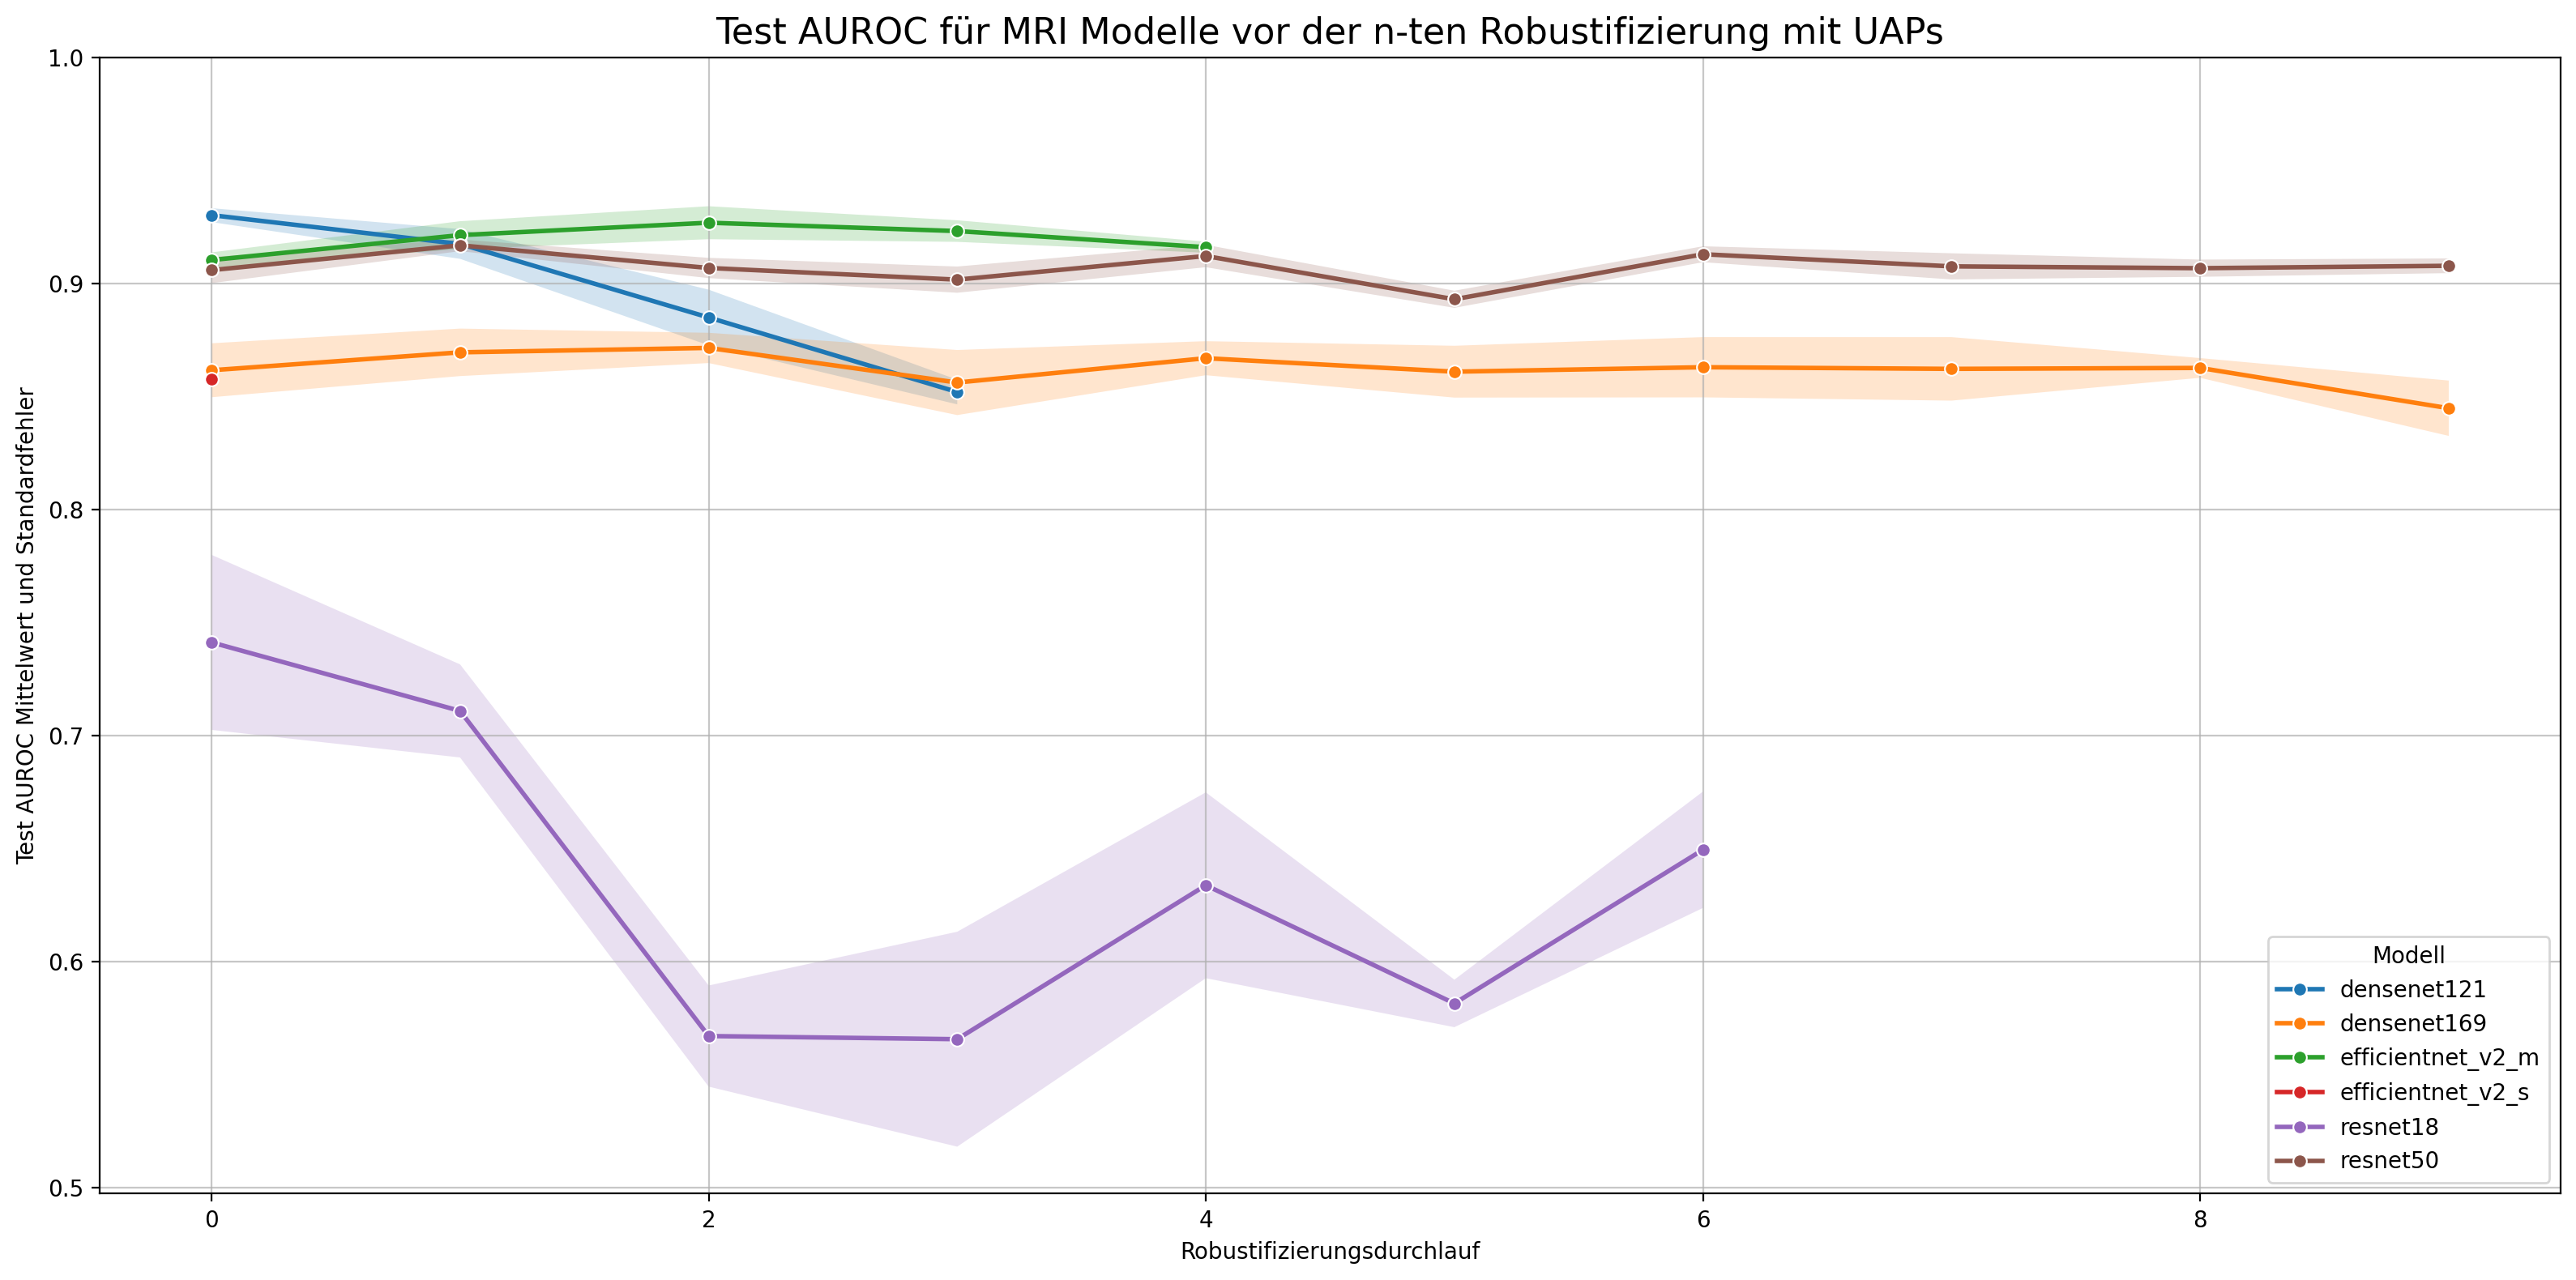
\includegraphics[width=\linewidth]{01-images/05-resultate/VerlaufAUROC_MRI.png}
    \caption{Verlauf der Test AUROC Metrik vor der n-ten \Gls{robustifizierung} für alle Modelle auf den MRI Datensatz}
    \label{fig:VerlaufAUROC_MRI}
\end{figure}

Bei der Abbildung \ref{fig:VerlaufAUROC_MRI} ist der Verlauf der Test-AUROC-Metrik während des Trainingsprozesses nach der Generation neuer \acrshort{uap}s und vor der Robustifikation dargestellt. Mit Ausnahme des bereits erwähnten ResNet18-Modells zeigt nur das DenseNet121-Modell eine stetige Verschlechterung der AUROC-Metrik mit jedem Robustifizierungsdurchlauf. Bei den übrigen Modellen bleibt die Leistung während des Prozesses weitgehend konstant. Bei keinem der Modelle ist eine Verbesserung hinsichtlich dieser Metrik festzustellen.

\subsubsection{COVIDx Datensatz}

Die Generation von \acrshort{uap}s, konnte auf nur 2 der 6 Modelle, welche auf den COVIDx Datensatz trainiert wurden, erfolgreich erschwert werden. Beide dieser Modelle sind DenseNet Modelle. Bei diesen Modellen erkennen wir verglichen zu den Modellen im MRI Datensatz nicht so deutlich, dass die Generierungszeit eines \acrshort{uap}s über den Robustifizierungsdurchlauf zugenommen hat. Verglichen zu den Modellen auf den MRI Datensatz wurden auch nicht sehr hohe Regularisierungsparameter gewählt.  

\begin{figure}[H]
    \centering
    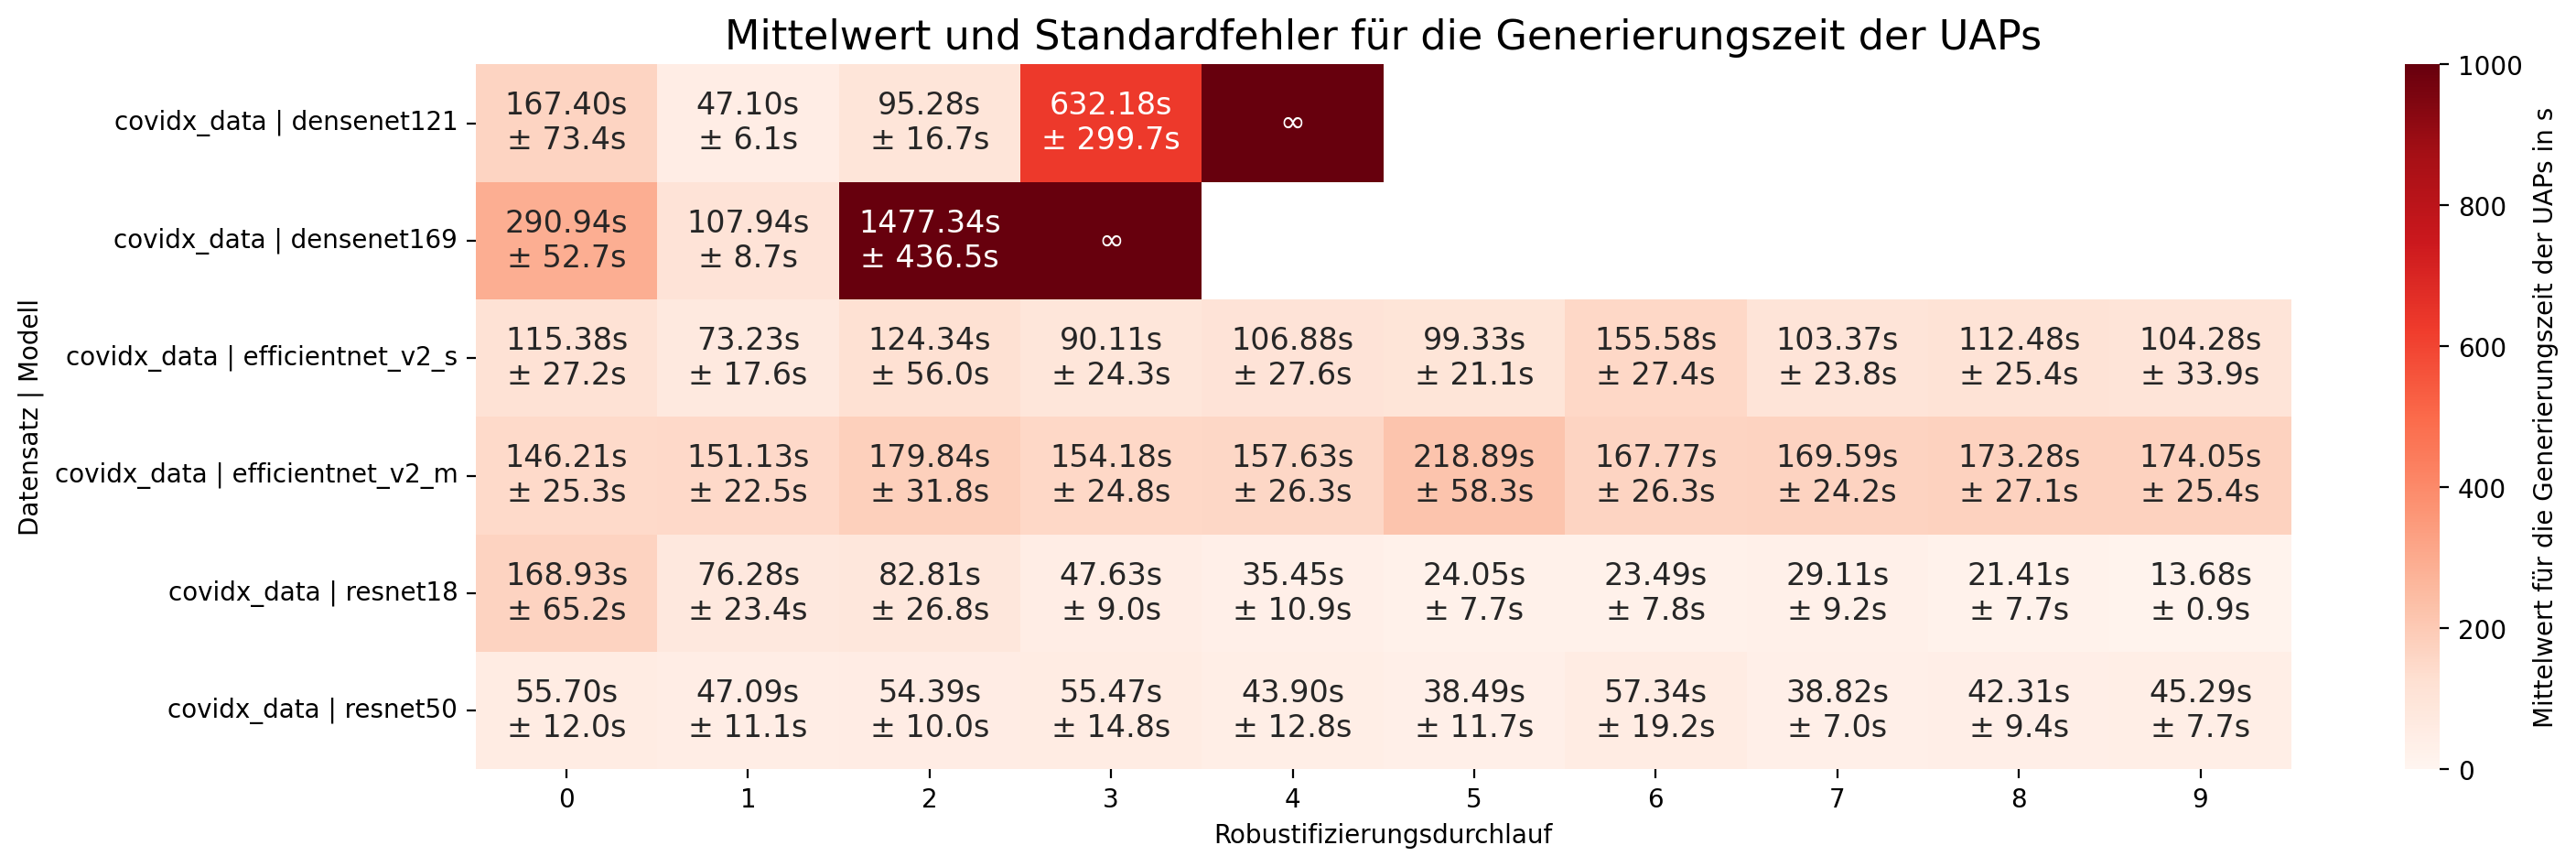
\includegraphics[width=\linewidth]{01-images/05-resultate/Generieungszeit COVIDx.png}
    \caption{Mittelwert und Standardfehler für die Generierungszeit der \acrshort{uap}s beim COVIDx Datensatz in Sekunden}
    \label{fig:GenerierungszeitUAPsCOVIDx}
\end{figure}


\paragraph{DenseNet}

% DenseNet121
\begin{figure}[H]
    \centering
    \foreach \y in {1} {%
        \text{Entwicklung der UAP (Index \y) durch Adversarial Attack und Adversarial Training}\\
        \foreach \x in {0,...,3} {%
            \ifnum\x>0 \hfill \fi 
            \begin{subfigure}{0.095\linewidth}
                \centering
                \includegraphics[height=1\linewidth]{01-images/05-resultate/uap_densenet121/uap\y-densenet121-covidx_data-n200-robustificationslevel\x.png}
            \end{subfigure}%
        }
    }
    \caption{UAPs der mit DenseNet121 trainierten Covid Datensatz nach jedem Robustifikationslevel durch Adversarial Training von links nach rechts}
    \label{fig:uap-densenet121-covid}
\end{figure}

Die durch das DenseNet121-Modell generierten \acrlong{uap}s (\acrshort{uap}s) zeigen, dass bei den ersten drei Robustifikationsstufen signifikante Perturbationen im oberen rechten Bereich auftreten. Diese Perturbationen werden mit zunehmender Robustifikationsstufe deutlicher und intensiver. Bereits ab der dritten Robustifikationsstufe treten mehrere dieser starken Perturbationen auf. In der letzten Perturbation sind weiterhin mehrere auffällige Cluster hoher Perturbationen auf der rechten Seite sichtbar. Generell sind die Perturbationen sowohl im negativen als auch im positiven Bereich stärker ausgeprägt. Im Vergleich zu den früheren Perturbationen sind diese deutlicher erkennbar, während die früheren Perturbationen kaum wahrnehmbar waren.

% DenseNet169
\begin{figure}[H]
    \centering
    \foreach \y in {0} {%
        \text{Entwicklung der UAP (Index \y) durch Adversarial Attack und Adversarial Training}\\
        \foreach \x in {0,...,2} {%
            \ifnum\x>0 \hfill \fi 
            \begin{subfigure}{0.095\linewidth}
                \centering
                \includegraphics[height=1\linewidth]{01-images/05-resultate/uap_densenet169/uap\y-densenet169-covidx_data-n200-robustificationslevel\x.png}
            \end{subfigure}%
        }
    }
    \caption{UAPs der mit DenseNet169 trainierten Covid Datensatz nach jedem Robustifikationslevel durch Adversarial Training von links nach rechts}
    \label{fig:uap-densenet169-covid}
\end{figure}

Analog zu den Ergebnissen beim DenseNet121-Modell zeigen die \acrlong{uap}s (\acrshort{uap}s) beim grösseren Modell, dem DenseNet169, ähnliche Muster. In der ersten \acrshort{uap} ist ebenfalls eine grössere Perturbation im oberen rechten Bereich zu erkennen, während kleinere Perturbationen fein über die gesamte \acrshort{uap} verteilt sind. In der zweiten Perturbation sind zwei signifikant stärkere Perturbationen sichtbar. Die erste aus der vorherigen Stufe ist weiterhin präsent und eine zweite grössere Perturbation ist weiter unten hinzugekommen. Mit der dritten Robustifikationsstufe sind die intensiven und signifikanten Perturbationen breiter verteilt und über die gesamte \acrshort{uap} hinweg sichtbar. Es gibt insgesamt mehr Perturbations- und Angriffsflächen bei dieser höheren Robustifikationsstufe.

\paragraph{EfficientNet}
% EfficientNet-V2-S
\begin{figure}[H]
    \centering
    \foreach \y in {0} {%
        \text{Entwicklung der UAP (Index \y) durch Adversarial Attack und Adversarial Training}\\
        \foreach \x in {0,...,9} {%
            \ifnum\x>0 \hfill \fi 
            \begin{subfigure}{0.095\linewidth}
                \centering
                \includegraphics[height=1\linewidth]{01-images/05-resultate/uap_efficientnet_s/uap\y-efficientnet_v2_s-covidx_data-n200-robustificationslevel\x.png}
            \end{subfigure}%
        }
    }
    \caption{UAPs der mit EfficientNetV2-S trainierten Covid Datensatz nach jedem Robustifikationslevel durch Adversarial Training von links nach rechts}
    \label{fig:uap-efficientnetv2s-covid}
\end{figure}

Beim Betrachten der universellen Adversarial Perturbation (\acrshort{uap}), die für EfficientNetV2-S und den COVID-Datensatz generiert wurde, sind horizontale Muster von positiven und negativen Perturbationen erkennbar. Diese Perturbationen variieren in ihrer Ausprägung je nach Robustifizierungslevel. Dies könnte darauf hindeuten, dass COVID-Bilder bei EfficientNetV2-S durch horizontale Muster leichter angreifbar sind.

% EfficientNet-V2-M
\begin{figure}[H]
    \centering
    \foreach \y in {1} {%
        \text{Entwicklung der UAP (Index \y) durch Adversarial Attack und Adversarial Training}\\
        \foreach \x in {0,...,9} {%
            \ifnum\x>0 \hfill \fi 
            \begin{subfigure}{0.095\linewidth}
            \centering\includegraphics[height=1\linewidth]{01-images/05-resultate/uap_efficientnet_m/uap\y-efficientnet_v2_m-covidx_data-n200-robustificationslevel\x.png}
            \end{subfigure}%
        }
    }
    \caption{UAPs der mit EfficientNetV2-M trainierten Covid Datensatz nach jedem Robustifikationslevel durch Adversarial Training von links nach rechts}
    \label{fig:uap-efficientnetv2m-covid}
\end{figure}

Die Perturbationen im Modell EfficientNetV2-M zeigen zwei auffällige Muster. Erstens erscheinen sowohl positive als auch negative Perturbationen in horizontalen, verwässerten Formen. Zweitens zeigt sich im unteren Bereich der universellen adversarialen Perturbation (\acrshort{uap}) ein vertikal alternierendes Muster von hohen und niedrigen Perturbationen. Diese hohen Perturbationen treten deutlicher hervor, je höher das Robustifikationslevel ist. Es scheint, dass die vertikalen Muster der Perturbationen hinter den horizontalen, verwässerten Mustern bedeckt sind.

\paragraph{ResNet}

% ResNet18
\begin{figure}[H]
    \centering
    \foreach \y in {3} {%
        \text{Entwicklung der UAP (Index \y) durch Adversarial Attack und Adversarial Training}\\
        \foreach \x in {0,...,9} {%
            \ifnum\x>0 \hfill \fi 
            \begin{subfigure}{0.095\linewidth}
                \centering
                \includegraphics[height=1\linewidth]{01-images/05-resultate/uap_resnet18/uap\y-resnet18-covidx_data-n200-robustificationslevel\x.png}
            \end{subfigure}%
        }
    }
    \caption{UAPs der mit ResNet18 trainierten Covid Datensatz nach jedem Robustifikationslevel durch Adversarial Training von links nach rechts}
    \label{fig:uap-resnet18-covid}
\end{figure}

Die Perturbationen für das Covid-Modell und das ResNet18-Modell zeigen spezifische Muster. In den ersten Robustifikationsstufen sind die universellen adversarialen Perturbationen (\acrshort{uap}) deutlich erkennbar. Besonders in den Randregionen treten Perturbationen in diagonalen Mustern auf. Im Zentrum hingegen sind die Perturbationen verteilt, während der untere mittlere Bereich der \acrshort{uap} keine starken Perturbationen aufweist. Mit steigendem Robustifikationslevel entwickeln sich in der oberen rechten Ecke wieder grössere Perturbationen, und alle anderen Perturbationen verteilen sich über die gesamte \acrshort{uap} hinweg.

% ResNet50
\begin{figure}[H]
    \centering
    \foreach \y in {2} {%
        \text{Entwicklung der UAP (Index \y) durch Adversarial Attack und Adversarial Training}\\
        \foreach \x in {0,...,9} {%
            \ifnum\x>0 \hfill \fi 
            \begin{subfigure}{0.095\linewidth}
                \centering
                \includegraphics[height=1\linewidth]{01-images/05-resultate/uap_resnet50/uap\y-resnet50-covidx_data-n200-robustificationslevel\x.png}
            \end{subfigure}%
        }
    }
    \caption{UAPs der mit ResNet50 trainierten Covid Datensatz nach jedem Robustifikationslevel durch Adversarial Training von links nach rechts}
    \label{fig:uap-resnet50-covid}
\end{figure}

Beim grösseren Modell, dem ResNet50, sind die Perturbationen über alle Robustifikationslevel hinweg konzentrierter. Es zeigt sich, dass insbesondere in der rechten oberen Ecke die Perturbationen deutlich hervortreten und sich dort konzentrieren. Abgesehen von dieser Region sind die restlichen Perturbationen fein verteilt und kaum vorhanden.

\paragraph{Zusammenfassung}
Bei der Analyse der \acrlong{uap}s (\acrshort{uap}) auf den COVIDx CXR-4 Datensatz zeigen sich modellabhängige Unterschiede in den Angriffsmustern.

Für das DenseNet-Modell, sowohl DenseNet121 als auch DenseNet169, konzentrieren sich die Perturbationen in der oberen rechten Ecke der Bilder. Diese gemeinsame Charakteristik deutet auf eine spezifische Schwachstelle in diesen Modellen hin.

Im Gegensatz dazu weisen die Perturbationen im EfficientNet-Modell stärkere und deutlich erkennbare Muster auf, einschliesslich horizontaler Linien und gemischter vertikaler Perturbationen. Die Angriffe sind somit breiter und verstreuter im Vergleich zu den DenseNet-Modellen.

Auch bei den ResNet-Modellen sind die Perturbationen in der oberen rechten Ecke der Bilder stark ausgeprägt, was auf eine ähnliche Schwachstelle wie bei den DenseNet-Modellen hinweist.

Es lässt sich feststellen, dass die \acrlong{uap}s je nach Modell unterschiedliche Muster aufweisen. Während die DenseNet- und ResNet-Modelle eine Präferenz für die obere rechte Bildregion zeigen, sind die Perturbationen beim EfficientNet-Modell breiter verteilt und durch spezifische Muster wie horizontale und vertikale Perturbationen charakterisiert. Diese Unterschiede unterstreichen die Notwendigkeit einer modellübergreifenden Analyse und Anpassung der Abwehrstrategien gegen \acrlong{uap} Attacks.

\begin{figure}[H]
    \centering
    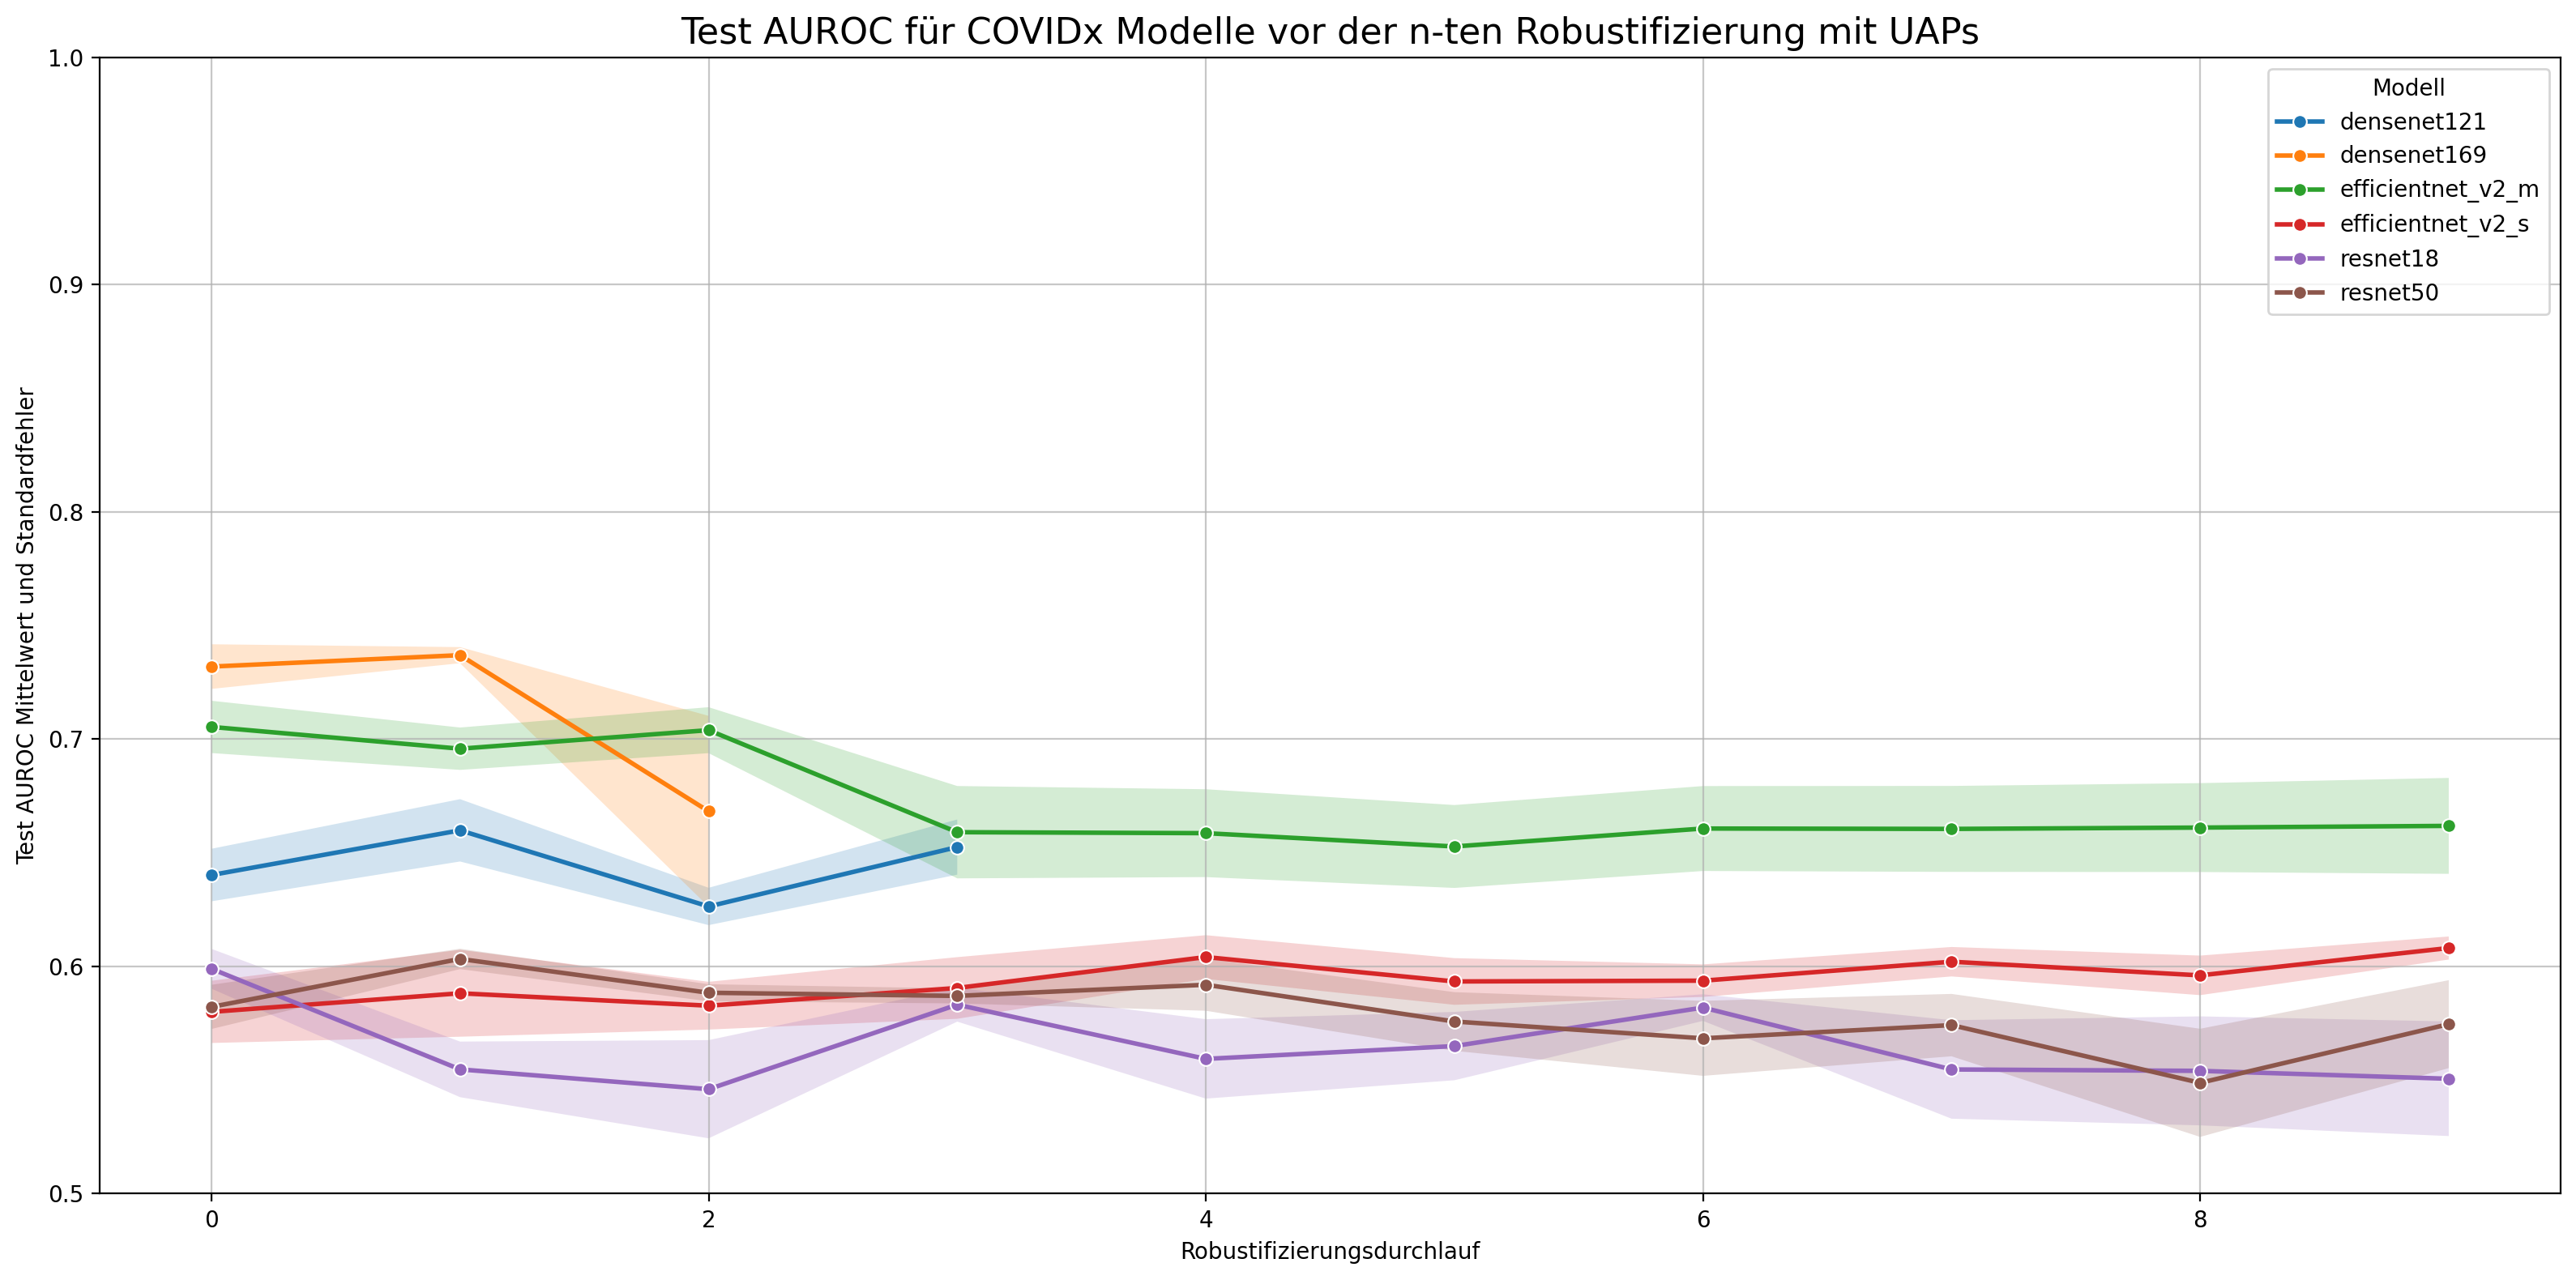
\includegraphics[width=\linewidth]{01-images/05-resultate/VerlaufAUROC_COVIDx.png}
    \caption{Verlauf der Test AUROC Metrik vor der n-ten \Gls{robustifizierung} für alle Modelle auf den COVIDx Datensatz}
    \label{fig:VerlaufAUROC COVIDx}
\end{figure}

Bei der Abbildung \ref{fig:VerlaufAUROC COVIDx} ist wie beim MRI Datensatz der Verlauf der Test-AUROC-Metrik während des Trainingsprozesses nach der Generation neuer \acrshort{uap}s und vor der Robustifikation dargestellt. Die Modelle DenseNet169, EfficientNetV2-M, ResNet18 und ResNet50 zeigen eine Verschlechterung der AUROC-Metrik über den Robustifizierungsprozess. Beim DenseNet121 und EfficientNetV2-S bleibt die Leistung während des Prozesses konstant oder steigt sogar minimal.

\subsubsection{Zusammenfassung}

Bei der Analyse konnte beobachtet werden, dass die \acrshort{uap}s pro Modell unterschiedlich erscheinen, jedoch diese \acrshort{uap}s beim gleichen Modell zwischen den Robustifizierungsdurchläufen Ähnlichkeiten aufweisen.

Die Addition einer \acrshort{uap} führt stets zur Verschlechterung der Recall-Metriken. Der ursprüngliche Zielwert der Metriken (ohne \acrshort{uap}s) kann durch \Gls{robustifizierung} oft nicht vollständig erreicht werden, was die Herausforderung der vollständigen \Gls{robustifizierung} unterstreicht.

Obwohl die \Gls{robustifizierung} auf den aktuellen \acrshort{uap}s hauptsächlich gut funktioniert, können neue \acrshort{uap}s generiert werden, welche das Modell ähnlich gut täuschen können wie die vorherigen Perturbationen vor der \Gls{robustifizierung}. Dies zeigt die fortwährende Anfälligkeit der Modelle gegenüber neuen \acrshort{uap}s.

Bei einigen Modellen funktioniert die \Gls{robustifizierung}, und die Perturbationen müssen grösser gemacht werden, damit sie das Modell weiterhin täuschen können, bis der aktuell gewählte Regularisierungsparameter zu hoch ist und das Modell keinen Angriff mehr generieren kann. Damit erhöht sich auch die Zeitintensität, diese \acrshort{uap}s zu generieren. Dies lässt sich jedoch mit dem Senken des Regularisierungsparameters und somit der Generation grösserer Perturbationen umgehen.

